\chapter{mD analysis with FMCW radar}
%Come è fatto questo capitolo
The previous chapter introduced the general characteristics of micro-Doppler analysis, the mathematical and theoretical tools needed to carry out the micro-Doppler study by means of a radar. The analysis is now focused on the specific case of the FMCW radar, which proves to be a hybrid instrument in this case. In fact, it can be used both in the case of the presence of range migration to perform the analysis on the Range-Time plane, being able to exploit the migration effect as an advantage. Or can be also used in conditions where migration is avoided, the classical analysis can be carried out on the Frequency-Time plane. The aim of this chapter is to investigate which of the two is the least expensive and most efficient finding a design compromise that ensures analysis on multiple drone models.\\
In the first part of the chapter we show the characteristics that can be extracted under ideal conditions from a spectrogram in the case of frequency-time analysis and from the range profile for the case of range-time analysis, respectively.\\
In the next part of the chapter, the construction parameters of an FMCW radar are investigated, and it is shown how they must be chosen so that the micro-Doppler information can be extracted without loss. The relationships between the radar parameters and the characteristic parameters of the targets to be observed with the mD analysis are made explicit. \\
In the next section, the signal model used before for a simple rotating point and then for an entire blade is shown. Based on the assumption of the scattering center model from a simple rotating point we can simulate an entire rotating object, such as a rotor's blade, considering multiple rotating point in sequence. In addition, the characteristic parameters to be entered in the model for each simulated drone are shown.\\
Then the received signal model is used as input of the FMCW radar processing chain by simulating the 2D FFT processing carried out by the radar with Matlab. The results obtained in the final part show that the signal model is compatible with the cause, allowing results similar to other signal models investigated in the literature such as \cite{microdoppler_chen}, \cite{kulpa}, \cite{MartinMulgrew}.\\
In the final part of the chapter, an optimisation algorithm for the waveform parameters simulated with Matlab is described, which allows the selection of the best waveform according to the desired minimum resolutions, both when the objective is range-time or frequency-time analysis.\\
Last, the results obtained with the different types of drones analysed both with and without cell migration are shown. It is possible at this point to decide which type of analysis is best to carry out in order to minimise costs. It is also possible to identify what type of design compromise can be made in order to be able to analyse several drone models with the same waveform.

\section{Features extraction}
%obiettivo estrarre informazioni per riconoscere il drone, mostrare adesso specificatamenete dove le pesco queste informazioni nei due casi rho t e ft esempi con immagini belle e precise (ideali)
The main objective of the micro Doppler study, as explained in detail so far, is to be able to recognise a drone in relation to other objects or birds. This is possible by recognising a characteristic frequency trend over time of the signal received by the radar due to the drone rotors. Not only is it possible to identify a drone by recognising the characteristic frequency trend, but it is also possible to obtain important information about the observed drone model. The characteristics on the observed object that can be identified are:

\begin{itemize}
     \item $\mathbf{T_{BF}}$: The period between two Blade Flashes (maximum mD contribution when the blade is perpendicular to the radar), the expression of which is typical of circular motion: 
     \begin{equation}
        T_{BF}=\frac{2 \pi}{N_{b} N_{r} \Omega}
        \label{BFperiod}
     \end{equation}
    Where $N_{b}$ is the number of blades in a rotor, $N_{r}$ is the number of rotors and $\Omega$ is rotation speed of the rotor. By inverting the expression \ref{BFperiod} and considering one single rotor it is possible to calculate the rotation speed $\Omega$ or the number of blades $N_{b}$ as follow:
    \begin{equation}
    N_{b}=\frac{2 \pi}{T_{BF} \Omega}
    \end{equation}
    \begin{equation}
    \Omega=\frac{2 \pi}{T_{BF} N_{b}}
    \end{equation}
         
    \item $\mathbf{N_{b}}$: It is also possible to determine whether the number of blades is odd or even by simply observing the composition of the sine waves in the plane. If, for example, the number of blades is even, each relative maximum will occur at the same time as a relative minimum. Maximums and minimums will therefore be coupled. On the contrary, when $N_{b}$ is odd, every relative maximum and minimum will occur in different temporal instants. An example of odd and even $N_{b}$ with related information is shown in the figures \ref{spect_helicopter_N_even} and \ref{spect_helicopter_N_odd}. In these figures the time period considered is that of a complete rotation of a single blade. Instead for convenience, for the purposes of this thesis, the time period between two blade flashes is always used;
    
    \begin{figure}[h!]
    \centering
    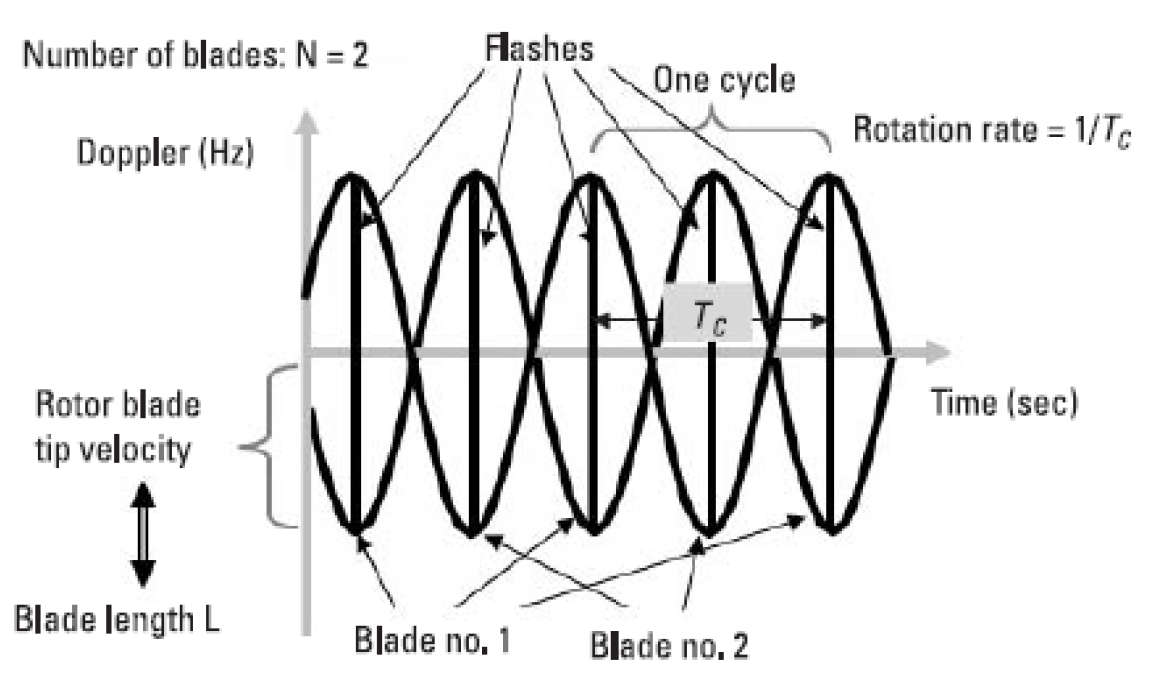
\includegraphics[width=10cm]{FMCW mD analysis-chap4/img/F-t plane md N even.png}
    \caption{Spectrogram of helicopter rotor blades with $N_b$ even. \cite{microdoppler_chen}}
    \label{spect_helicopter_N_even}
    \end{figure}
    
    \begin{figure}[h!]
    \centering
    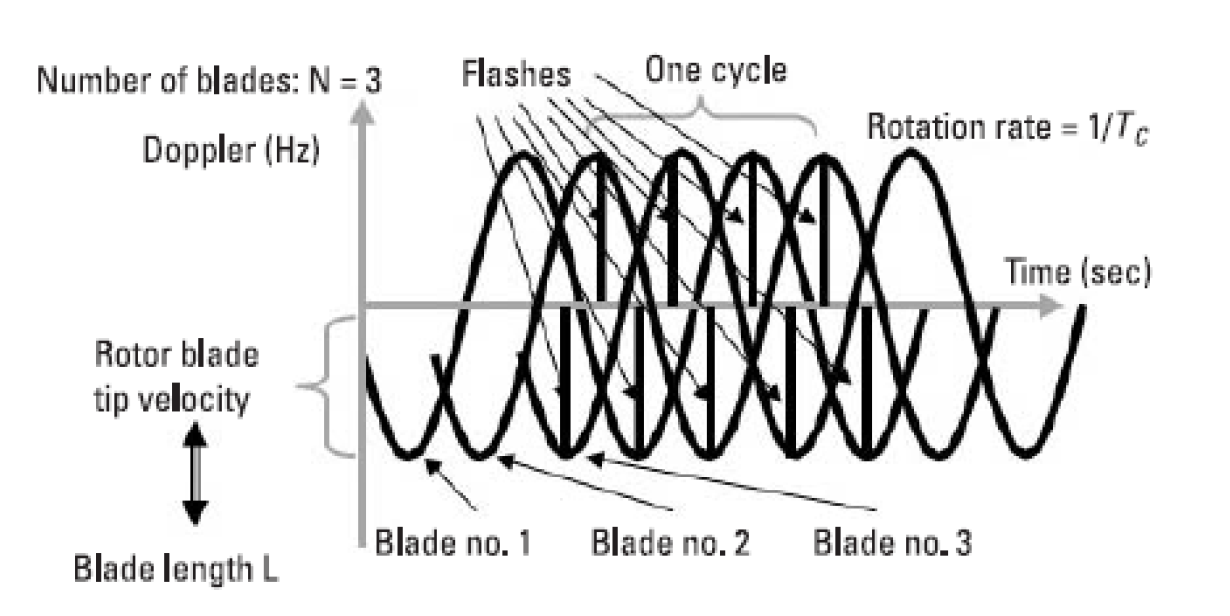
\includegraphics[width=11cm]{FMCW mD analysis-chap4/img/f-t plane md N odd.png}
    \caption{Spectrogram of helicopter rotor blades with $N_b$ odd. \cite{microdoppler_chen}}
    \label{spect_helicopter_N_odd}
    \end{figure}
    
    \item $\mathbf{L}$: The length of a blade is an information that can be extracted from knowledge of the maximum excursion in frequency denoted as $f_{D, max}$ or in range denoted as $R_{migr, max}$, depending on the plane in which the analysis is. In the first case we have:
    \begin{equation}
    L=\lambda \frac{f_{D, \max }}{2 \Omega}
    \end{equation}
    It is possible to visualize this information on the y-axis of both previous figures (\ref{spect_helicopter_N_even} and \ref{spect_helicopter_N_odd}). \\
    While in the range-time plane we have:
    \begin{equation}
    L=\lambda \frac{R_{max} \lambda \mu}{\Omega c}
    \label{L_rho_t}
    \end{equation}
    The ideal trend of range variation of a rotor as studied in \cite{microdoppler_chen} is shown in figure \ref{r-t_2_points}.
    
    \begin{figure}[h!]
    \centering
    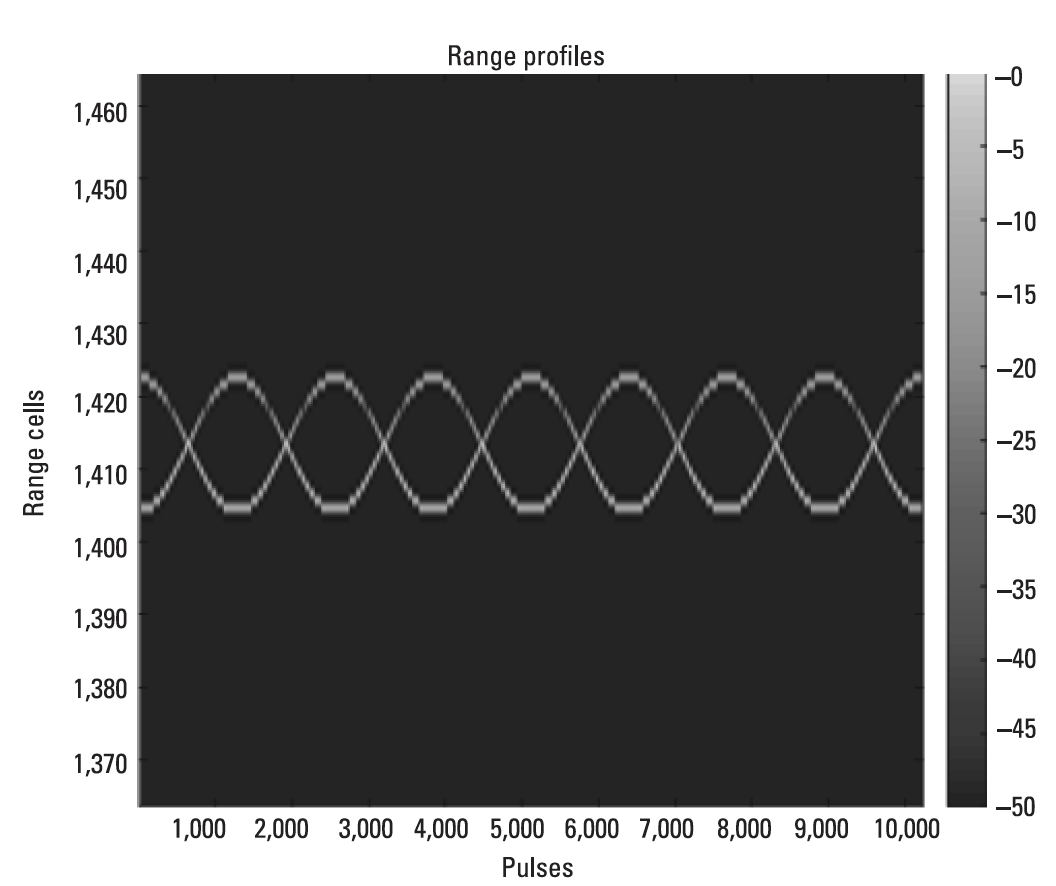
\includegraphics[width=11cm]{FMCW mD analysis-chap4/img/Range profile variations chen.png}
    \caption{Range profile of 2 rotating points.}
    \label{r-t_2_points}
    \end{figure}
    
    In this case two rotating blades are approximated as two rotating points with respect to their centre of rotation located approximately in the range cell 1415. It is possible to observe the variation that occurs quantified in number of migrating cells with respect to the centre of the rotor.\\ 
    In order to better visualize the ideal trend of range-time variations, simulating with Matlab the equation of the range variations for 2 rotating points (\ref{range_var_1}), we obtain the figure \ref{r-t_helicopter_N_odd}. Each point is in opposite respect to the other and represent the blade's tip. The length of the blade extracted from the maximum range of the signal received by the target is shown. The relationship for calculating the period between two blade flashes remains the same as in the case of time-frequency analysis (\ref{BFperiod}).
    
    \begin{figure}[h!]
    \centering
    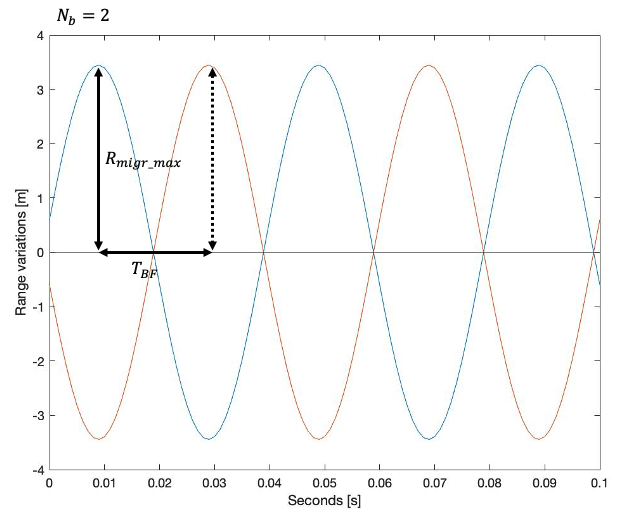
\includegraphics[width=11cm]{FMCW mD analysis-chap4/img/rho-t plane features.png}
    \caption{Range profile of helicopter rotor blades with $N_b$ = 2.}
    \label{r-t_helicopter_N_odd}
    \end{figure}
    
    The value of L in this case is obtained by measuring the max value of R, denoted as $R_{migr, max}$ and considering that from (\ref{range_var_1}) the maximum is:
    \begin{equation}
    R_{migr, \max }=\frac{c L \Omega}{\lambda \mu}   
    \label{Rmigrmax}
    \end{equation} 
     Where $\mu$ is the radar slope, $c$ is the speed of light and $\lambda$ is the wavelength. The previous considerations regarding the number of blades making up a rotor also apply here, if they are even or odd.
  
\end{itemize}

At the end of the feature extraction, it is possible to know the time period between two blade flashes, the length of the rotating blade, the number of rotating blades and the rotation speed, making it possible to at least recognise the type of drone observed or even better to recognise the specific model of drone. At least is possible to distinguish the two macro categories of drones, quadcopters and helicopters. The quadcopter drone is usually characterised by four different rotors, each containing two blades. In addition, the length of the blades is much shorter than that of the helicopter drone and the rotation speed is higher. The helicopter drone, on the other hand, is characterised by a single rotor with at least two blades. 
The next sub-section shows the ideal spectrogram and range profile trends for the two different drone types.

\subsection{Helicopter drone}
Having seen the ideal case of spectrograms and range profiles for a single rotor with two or more blades, the simulated spectrogram and range profile trends for a helicopter drone are now shown under ideal conditions. In this way, the features just shown can be clearly appreciated. The following figure \ref{ideal_helic_spect} shows the spectrogram of a helicopter drone simulated under ideal conditions, i.e. using a waveform that is not compatible with a specific radar but only selected in order to best observe the drone's characteristics. Also the number of samples in a STFT window is chosen only to improve the resolution without considering any design parameter. 

\begin{figure}[h!]
\centering
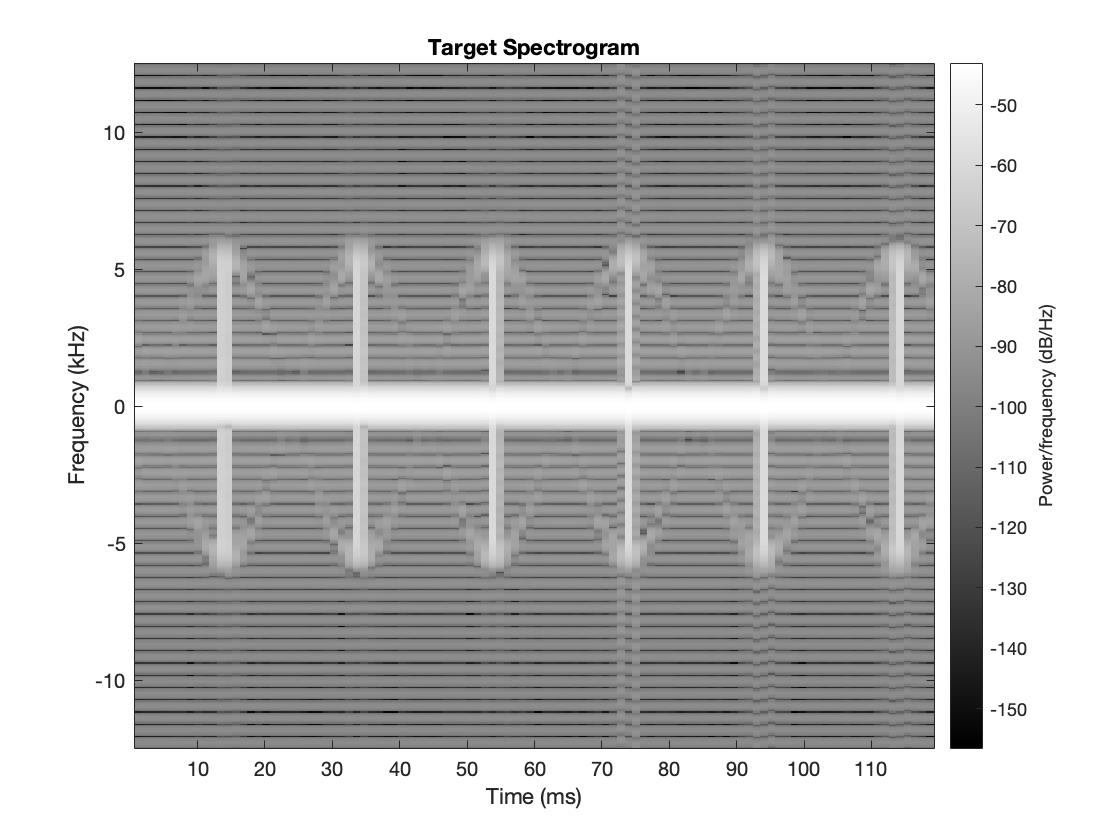
\includegraphics[width=10cm]{FMCW mD analysis-chap4/img/helicopter_ideal_spectrogram.jpg}
\caption{Helicopter drone spectrogram under ideal conditions.\cite{tesiligresti}}
\label{ideal_helic_spect}
\end{figure}

For this ideal representation, the central body of the drone was considered as $25\%$ of the total RCS of a drone. The signal received by the blades was derived from the models \cite{kulpa}, \cite{microdoppler_chen} and all the work has been extensively described in \cite{tesiligresti}. It is very clear in this case how all the information listed above can be easily seen and appreciated.\\
With regard to the range profile of a helicopter drone under conditions of cell migration in ideal case, it is possible to observe the figures shown above, \ref{r-t_helicopter_N_odd} and \ref{r-t_2_points}. In particular in the \ref{r-t_helicopter_N_odd} it is possible to observe the constant contribution due to the body of the drone as the fixed black line. 
It is important to consider that in this ideal case the drone body has been approximated simply as a single reflecting point as well as the two rotor blades have been considered as two rotating points at distance $L$ from the rotor. In pratictice we are simulating the effect of the blade tip, the point that has the highest velocity and consequently makes the greatest Doppler shift and range migration. So all the other points that make up the rotating blade are below them and will have a lower speed. Furthermore, this approximation is compatible with the scattering centre model, thus making these initial simulations a starting point for real cases. These coarse representations make it possible to understand what is expected to be observed in broad terms in the case of a real range profile.
Another important assumption that allows us to focus only on the rotational motion of the blades is to consider the drone in a hovering state.

The objective will be to go from an ideal case to a real case and to be able to observe all the features shown without loss of information.

\subsection{Quadcopter drone}
The next figure \ref{ideal_quad_spect} shows the spectrogram of a quadcopter drone simulated under ideal conditions, as in the previous case with reference to the discussion in \cite{tesiligresti}. Again, the waveform parameters used and the number of samples taken in a window of the STFT is aimed at the only benefit of visualisation, without considering any design requirements.

\begin{figure}[h!]
\centering
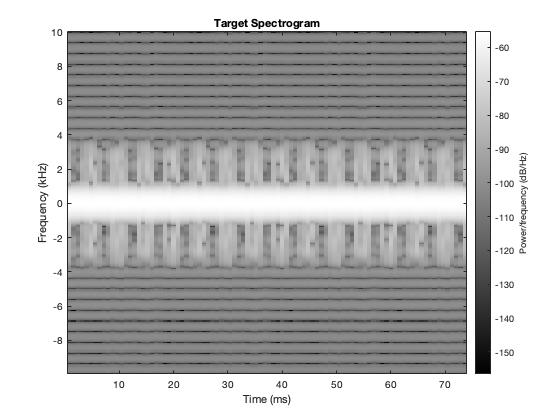
\includegraphics[width=10cm]{FMCW mD analysis-chap4/img/quad_ideal_spect.jpg}
\caption{Quadcopter drone spectrogram under ideal conditions.\cite{tesiligresti}}
\label{ideal_quad_spect}
\end{figure}

In this case, it is possible to observe that blade flashes are much more frequent, due to the presence of four rotors, each with two blades. However, it remains clearly visible that the necessary information is easily extractable and visible, such as the period between two blade flashes or the maximum Doppler frequency.\\
With regard to the ideal representations of the range profile for a quadcopter drone, as in the previous case, the same rough approximation is made in order to roughly understand the trend that is expected to be observed in reality. The body of the drone is considered as a reflective point and the two blades of each rotors are approximated as the respective blade's tip points. As described before, simulating the equation of range cell migration (\ref{range_var_1}), the figure \ref{quad_r_t_ideal} shows the ideal trend of a quadcopter drone observed in the range-time plane.

\begin{figure}[h!]
\centering
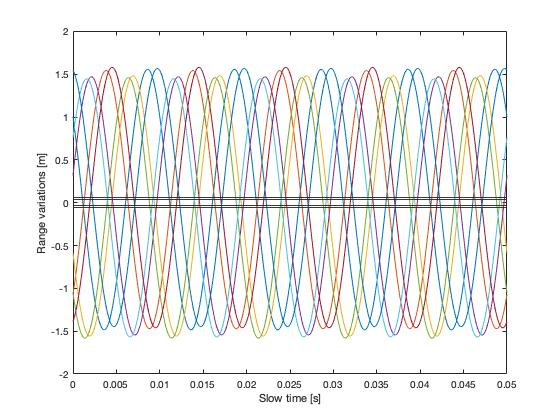
\includegraphics[width=11cm]{FMCW mD analysis-chap4/img/quad_r_t_ideal.jpg}
\caption{Quadcopter ideal range profile simulated from theoretical formula.}
\label{quad_r_t_ideal}
\end{figure}

In this case the black lines are that of rotor position, and take into account the different position of the rotors in pairs with respect to the elevation angle.
Considering that in this simplified ideal case where the blades are approximated by single points, the result still appears very dense. This indicates that in the real case one expects to obtain a result that is not as clear as in the case of a helicopter drone. In fact, the same thing happens for the spectrogram of a quadcopter drone compared to that of a helicopter drone. This is due to the presence of several rotors characterised by a shorter period between blade flasehs.



\section{Radar design}
%Obiettivo voler osservare senza perdere informazione i piani rho t e f t senza perdere troppa informazione. Quindi Come scelgo i parametri del radar FMCW inizio fase di design, parto sempre dalla radar equation e dalla potenza poi Contraint generali del radar ( sui parametri) e limiti sul radar imposti dal target che si vuole osservare
The design phase involves choosing the specifications that the radar must meet and by determining its dimensions with the aim of being able to maintain adequate time and frequency resolution considering the characteristics of the target. The design is considered satisfactory if the information shown above under ideal conditions on the planes Range-Time and Frequency-Time can be appreciated by the radar. The main objective of this step is to correctly determine the duration of the transmitted chirps and all the other radar parameters since, as shown below, there are a number of limitations imposed by the performance requirements on these. 

\subsection{Radar parameters}
The requirements to be met by the radar in general depend on the performace that must be achieved and on target features, there are several ways of determining these, in general the main limitations to be taken into account come from the follow parameters:
\begin{itemize}
    \item \textbf{$R_{max}$}: maximum detection range;
    
    \item \textbf{$v_{max}$}: maximum velocity to be measured;
         
    \item \textbf{$\Delta r$}: desired resolution in range;
    
    \item \textbf{$\Delta f$}: desired resolution in frequency;
\end{itemize}
Given $R_{max}$ at which the presence of a drone is to be detected, the main limitation resulting from this is the range ambiguity. To avoid ambiguity in range, the ramp duration must be at least $\mathrm{k}$ times longer than the maximum propagation 2-way delay from that distance. Result the relationship \ref{chirp_min_by_range} where $\mathrm{k}$ is usually at least 10 and $c$ is the light speed:
\begin{equation}
T_{\text {chirp}}>\mathrm{k} \frac{2 R_{\max }}{c}
\label{chirp_min_by_range}
\end{equation}
Another important requirement depending on the maximum distance is the link budget, so the necessary power that radar must transmit per ramp. In the following equation \ref{surveillance_radar_eq} this dependence is shown through the surveillance equation in the case of a continuous wave radar:
\begin{equation}
\mathrm{R}_{\max }=\left(\frac{\sigma P_{t} G_{T X} G_{R X} \lambda^{2} NT_{\text {chirp }}}{(4 \pi)^{3} S N R_{\min } k T F}\right)^{\frac{1}{4}}
\label{surveillance_radar_eq}
\end{equation}

\begin{itemize}
    \item \textbf{$G$}: represents the antenna gain that depends on the beam size in azimuth and elevation;
    
    \item \textbf{$P_{t}$}: represents the power transmitted by the radar;
         
    \item \textbf{$\sigma$}: represents the power transmitted by the radar; sigma is the RCS of the target;
    
    \item \textbf{$\lambda$}: is the wavelength;
    
    \item \textbf{$N$}: is the number of ramps on the target during the observation time;
    
    \item \textbf{$T_{chirp}$}: is the duration of each individual ramp;
    
    \item \textbf{$T$}:  is the system temperature;
    
    \item \textbf{$F$}:  is the noise figure;


\end{itemize}


This requirement varies greatly if the analysis is to be carried out in the f-t plane or in the R-t plane. The difference lies in the fact that in order to conduct the analysis in the frequency plane, no cell migration must be present, so that coherent integration between all chirps sent to the target during the observation time is possible. The energy to be transmitted associated with each ramp thus becomes very small. If, on the other hand, the analysis is to be conducted in the range-time plane, it is not possible to perform coherent integration between the various chirps received due to the migration effect. Consequently, all the energy required to meet the $SNR_{min}$ requirement must be associated with each individual ramp and cannot be divided per each ramp into the dwell time. It is like to observe the equation (\ref{surveillance_radar_eq}) with $N=1$. This fact is one of the two most important difference between the two analysis, it shows that the analysis in the f-t plane is less demanding in terms of transmitted power. \\
The maximum speed to be measured $v_{max}$, as anticipated, depends on the measurements made on the phase, which are only disambiguous for variations less than $\pi$. As shown in detail with all the steps in \cite{2Dprocessing_fmcw}, the maximum speed that can be measured disambiguously is as follows:
\begin{equation}
v_{\max }=\frac{\lambda}{4 T_{chirp}}
\label{vmax}
\end{equation}
Considering the relation among velocity and frequency:
\begin{equation}
f_{\max }=\frac{2 v_{max}}{\lambda}
\label{fmax}
\end{equation}
Inserting \ref{fmax} in \ref{vmax} we obtain the following limations on chirp duration:
\begin{equation}
T_{chirp}<\frac{1}{2 f_{max}}
\label{chirp_max_lim_by_vel}
\end{equation}
The \ref{chirp_max_lim_by_vel} represents the most stringent limitation on the duration of the waveform, as the resulting values are often very small considering the high speeds reached by the rotating blade tips. Having a low chirp time duration could lead to an increase in the radar's slope parameter, which as we shall see later is directly reflected in the required sampling frequency. This limitation is completely avoided if the analysis is to be conducted on the range-time plane, as it would no longer be necessary to measure velocities. It is very important to keep this relationship in mind as it represents the second most important difference between the two analyses conducted on the two different planes, along with the power requirement.\\
The desired range resolution determines the band required by the radar according to the relationship:
\begin{equation}
B=\frac{c}{2 \Delta r}
\end{equation}

In addition, it is important to remember that the band is required to determine the radar slope $S = B/T_{chirp}$.\\ 
Another important parameter is the required sampling rate that depends on the parameters seen so far.
\begin{equation}
f_{ADC }= 2 (\frac{S 2 R_{\max }}{c}+\frac{2 v_{max}}{\lambda})
\label{samplingfreq}
\end{equation}
If it is too high, it could become limiting to the realisation of the radar.\\
The last general parameter mentioned so far is the frequency resolution, in case of FMCW it is inverse proportional to the time spent on target, so it result in a limitation on the dwell time:
\begin{equation}
\Delta f= \frac{1}{t_{dwell}}
\end{equation}

\subsection{Resolutions parameters for target classification}
The resolution parameters depend on the characteristics of the drones to be observed and are different depending on the plane in which the analysis is to be conducted. In both cases, limitations are imposed on the duration of the chirp signal, the observation time and on the length of FFT windows used during the processing. In this phase, the limits that must be respected for the features on the two planes to be extractable are determined. Consequently, these limitations concern the possibility of being able to perform recognition. Whereas in the previous phase, the limitations mainly concern the possibility of being able to perform the detection. The case of the range-time analysis is shown below, followed by the frequency-time analysis.
\subsubsection{Range-time resolutions}
In the case of the Range-Time analysis, the resolutions involved are the distance and the time resolutions, the first is fixed by the chosen bandwidth. The temporal resolution in this case is given by the window of the FFT used to estimate the max frequency of each ramp. Since an FFT is done for each ramp of duration $T_{chirp}$, the time resolution is precisely $\Delta t = T_{chirp}$. In figure \ref{ideal_r_t_res} is shown the theoretical simulation of range variation of an helicopter drone, as described before. In the example the range resolution is $ \Delta r = 0.2\; m$ and the time resolution is $\Delta t = 2 \; ms$. While the simulated drone parameters are the ones showed in the previous table \ref{vel_table}.

\begin{figure}[h!]
\centering
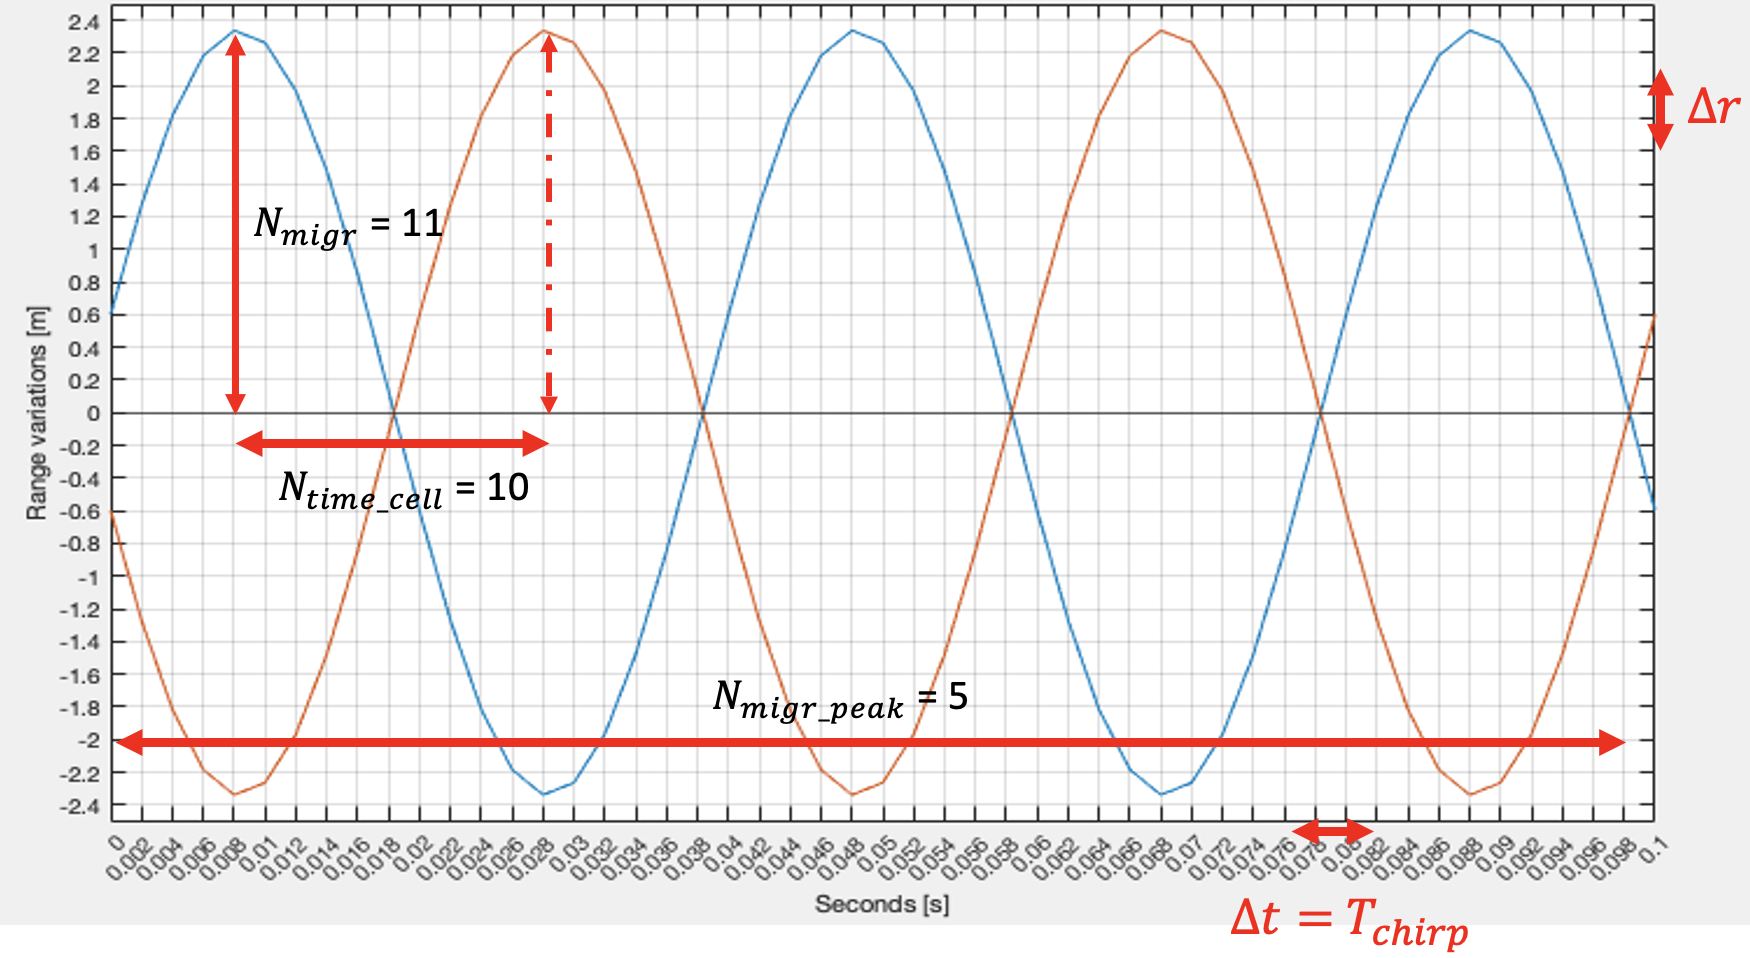
\includegraphics[width=12cm]{FMCW mD analysis-chap4/img/resolution in ro.t.png}
\caption{Range-Time plane with resolutions}
\label{ideal_r_t_res}
\end{figure}

Now it's possible to visualize the grid of resolutions composed by $\Delta r$ and $\Delta t$ pixels. 
Having defined the resolutions and having the graphical visualisation available, it is easier now to define the limitations that are imposed on the radar parameters due to the resolution requirements so that the peaks can be appreciated and distinguishable from each other. By defining how many time pixels are at least required between two consecutive blade flashes as $N_{time-cell}$, and defining how many pixels in distance are at least required below a peak as $N_{range-cell}$, the following limitations are determined. In figure \ref{ideal_r_t_res} the range cell migrated are denoted by the vertical red line, while the range time cell between two blade flash are denoted by the horizontal red line. As done to derive the condition to be imposed on the duration of the chirp to avoid migration in the \ref{chirpmigrationcond}, on the contrary now we want to emphasise this aspect. We no longer choose to limit the number of migrated cells below one, but instead impose that the number of migrated cells in the maxima must be at least greater than $N_{range-cell}$.
\begin{equation}
N_{\text {migr }}=\frac{R_{\text {migr-max }}}{\Delta r}>N_{\text {range-cell }}
\label{mincellmigration}
\end{equation}
Where $N_{migr}$ is the number of cell migrated under a peak, defined as the maximum of range migration denoted as $R_{migr-max}$ divided by the length of each cell. Considering the expression of $R_{migr-max}$ as showed in (\ref{Rmigrmax}) inserting in (\ref{mincellmigration}) we obtain:
\begin{equation}
T_{\text {chirp }}>\frac{\lambda N_{range-cell }}{2 L \Omega}
\label{min_chirp_by_res_rt}
\end{equation}
That is a lower limitation imposed to the chirp duration.\\
Regarding the number of time cells desired between two blade flashes, it define the required time resolution:
\begin{equation}
\Delta t_{req} = \frac{T_{BF}}{N_{time-cell}}
\label{time_res_req_rt}
\end{equation}

Considering that the time resolution is equal to the duration of the chirp and that at least $N_{time-cell}$ are desired, the following relationship follows:
\begin{equation}
T_{chirp}<\frac{T_{BF}}{N_{time-cell}}
\label{time_cell_limit}
\end{equation}
Inserting the expression of $T_{BF}$ (\ref{BFperiod}) we obtain:
\begin{equation}
T_{chirp}<\frac{2 \pi}{N_{b} \Omega N_{time-cell}}
\label{max_chirp_rt}
\end{equation}
That is an upper limitation imposed to the chirp duration.\\
Another important constraint to consider coming by determining the minimum number of peaks that are at least visible in the plane denoted as $N_{peak}$. This assumption is mapped to a limitation on the dwell time as follow:
\begin{equation}
t_{dwell}>\frac{2 \pi N_{\text {peak }}}{N_{b} \Omega}
\label{dwell_rt_limit}
\end{equation}
That is the minimun time to spent on target during one observation in order to visualize $N_{peak}$ variations.\\
At the end if we consider both the limitation imposed by the radar parameters and by the resolution parameters to the chirp duration we obtain two intervals, the first:
\begin{equation}
k \frac{2R_{max}}{c}<T_{chirp}<\frac{1}{2 f_{max}}
\label{radar_limit_interval}
\end{equation}
The (\ref{radar_limit_interval}) shows the interval of $T_{chirp}$ values compatible with radar parameters in order to correct detect an object at distance $R_{max}$ and to detect without ambiguity the micro-Doppler frequencies. The second interval:
\begin{equation}
\frac{\lambda N_{range-cell }}{2 L \Omega}<T_{chirp}<\frac{2 \pi}{N_{b} \Omega N_{time-cell}}
\label{resolution_limit_interval}
\end{equation}
The (\ref{resolution_limit_interval}) shows the interval of $T_{chirp}$ values compatible with desired resolutions necessary to observe a drone with at least $N_{time-cell}$ between two consecutive blade flash and at least $N_{range-cell }$ below a maximum of range variation. The intersection between these two intervals determines the existence range of $T_{chirp}$ values compatible with both the radar and the targets to be observed.\\
To sum up in the end we have 3 different intervals for the possible values of $T_{chirp}$:

\begin{itemize}
    \item The (\ref{radar_limit_interval}): allows the target to be correctly detected;
    
    \item The (\ref{resolution_limit_interval}): makes it possible to identify the typical micro-Doppler trend on the Range-Time plane;
         
    \item The third: the intersection between the two, allows both tasks to be performed.

\end{itemize}

\subsubsection{Frequqency-time resolutions}
In the case of time-frequency analysis the resolutions in question are as usual the temporal one $\Delta t$ and in this case the frequency one $\Delta f$. Recalling the logical procedure of the STFT that is the tool used to construct the spectrogram and analyse the signal in the f-t plane. The temporal resolution is given by the width of the FFT window used. In particular, as explained in Chapter 3, the chosen FFT window of width $N_{fft}$ is shifted on the signal by $N_{fft}/2$ at a time. Consequently, the resulting temporal resolution will be:
\begin{equation}
\Delta t=\frac{N_{fft} T_{chirp}}{2}
\label{temporal-ft-res}
\end{equation}
While frequency resolution is inversely proportional to the time spent on the target. So, since the time spent on the target in each STFT transform is equal to the number of chirps taken in a window, we have:
\begin{equation}
\Delta f=\frac{1}{N_{fft} T_{\text {chirp }}}
\label{freqeuncy-ft-res}
\end{equation}
As in the previous case, these quantities form a grid of pixels and it then becomes possible to define how many pixels are required between two blade flashes and below each maximum for features to be easily extracted. By defining the minimum number of pixels required between two blade flashes as $n_{t}$, the following relationship is obtained:
\begin{equation}
\Delta t_{req}=\frac{T_{BF}}{n_{t}} 
\label{time-res-ft}
\end{equation}
The (\ref{time-res-ft}) is the required time resolution.
Considering that to have at least $n_{t}$ time pixel between two blade flash, and considering the $T_{BF}$ expression as previous, we obtain the following limitation imposed on $T_{chirp}$:
\begin{equation}
T_{chirp}<\frac{4 \pi}{n_{t} N_{fft} N_{b} \Omega}
\label{upper_chirp_limit_ft}
\end{equation}
Where $N_{b}$ is the number of blades in a rotor. The (\ref{upper_chirp_limit_ft}) represents an upper limit imposed on chirp duration. \\
Now defining the minimum number of pixels required under a maximum as $n_{f}$ we obtain the following relationship:
\begin{equation}
\Delta f_{req}=\frac{f_{max}}{n_{f}} 
\label{freq-res-ft}
\end{equation}
Equation (\ref{freq-res-ft}) is the required frequency resolution.
Considering that to have at least $n_{f}$ frequency pixels between two blade flash, we obtain the following limitation imposed on $T_{chirp}$:
\begin{equation}
T_{chirp}>\frac{n_{f}}{N_{fft} f_{\max }}
\label{lower_chirp_limit_ft}
\end{equation}
The (\ref{lower_chirp_limit_ft}) represents a lower limit imposed on chirp duration. As in the previous case, considering together the limitations imposed on the chirp duration by the radar parameters and by the required resolutions, we have two intervals, the first is given by (\ref{radar_limit_interval}). The second is:
\begin{equation}
\frac{1}{N_{fft} \Delta f_{\text {req }}}<T_{\text {chirp }}<\frac{2 \Delta t_{\text {req }}}{N_{fft}}
\label{res_interval_ft}
\end{equation}
The (\ref{res_interval_ft}) represents all possible values of the chirp duration that satisfy the resolution requirements, which thus enable identification to be carried out correctly. Whereas, as explained earlier, the first interval (\ref{radar_limit_interval}) represents all values of the chirp duration that satisfy the radar requirements, which thus enable detection to be carried out correctly. The intersection between the two ranges represents all values that satisfy both radar and resolution requirements, making both detection and identification possible.



\section{Drone's signal model}
%Modello del drone partendo dalla formula generale dopo il battimento per un singolo punto poi estesa a 100 punti, tabella in cui inserisco ogni drone con le sue caratteristiche, compatibilità con modelli derivati dallo stop go ( i risultati senza migrazione sono uguali)
%Tabella con parametri di ogni drone
The received signal model from the drone used for the simulations is shown below. The signal is derived in successive steps. The starting point is given by the equation of the chirp signal received by the radar from a certain distance $R$, as described extensively in Chapter 3 and showed in the formula (\ref{beatstopgomodel}), after the dechirping operation that took plane in the FMCW radar, we have the following signal:

\begin{equation}
\begin{aligned}
s_{R}(t)=& \operatorname{rect}\left(\frac{t_{f}-2 R\left(t_{s}\right) / c}{T_{c}}\right) \\
& \cdot \exp \left(j\left(-\frac{4 \pi}{c} \mu t_{f} R\left(t_{s}\right)-\frac{4 \pi}{c} f_{c} R\left(t_{s}\right)+\frac{4 \pi \mu}{c^{2}} R\left(t_{s}\right)^{2}\right)\right)
\end{aligned}
\label{start_formula_model_signal}
\end{equation}

\begin{itemize}
    \item $\mu$  is the radar slope;
    
    \item $c$ is the light speed;
         
    \item $T_{c}$ is the chirp duration;

    \item $f_{c}$ is the center frequency;

\end{itemize}

It's important to note that the time instants $t_{f}$ relative to the exponential terms are in the fast time domain, as we are interested in the migrations that occur in this time frame.
$R(t_s)$ is the equation of the motion of the target and its time instants $t_{s}$ are in the slow time domain, because we must consider the motion evolution during all the processing time.\\
The first step is to consider a single rotating point whose equation of motion, as already seen, is:
\begin{equation}
R_{point}(t_s)=R_{0}+\rho \cos \left(\Omega t_{s}+\theta_{0}\right)
\end{equation}
In this case we are considering only the rotational motion, the trasnlatory motion is considered separately.
The idea is to consider this first point as the blade tip point, whose distance from the centre of rotor is $\rho$ and its rotation rate is $\Omega$. Starting from the blade tip point it's possible to consider the blade composed by infinitesimal points. The total received signal from the blade is a summation of all the infinitesimal points contributions. The \ref{start_formula_model_signal} can be rewritten as follow: 
\begin{equation}
\begin{aligned}
s_{R}(t)=& \sqrt{\sigma_{point}} \int_{L_{2}}^{L_{1}}\operatorname{rect}\left(\frac{t_{f}-2 R_{point}\left(t_{s}\right) / c}{T_{c}}\right) \\
& \cdot \exp \left(j\left(-\frac{4 \pi}{c} \mu t_{f} R_{point}\left(t_{s}\right)-\frac{4 \pi}{c} f_{c} R_{point}\left(t_{s}\right)+\frac{4 \pi \mu}{c^{2}} R_{point}\left(t_{s}\right)^{2}\right)\right) d\rho
\end{aligned}
\label{step2_formula_model_signal}
\end{equation}

In \ref{step2_formula_model_signal} it is added also the RCS point contribution. The novelty is introduced by the integral that goes from $L_{1}$ to $L_{2}$, where:
\begin{itemize}
    \item $L_{1}$ is the blade root position;
    
    \item $L_{2}$ is the blade tip position;
         
\end{itemize}
Moving to the discrete world it's possible to consider the integral as a summation of each point that make up the blade according with the scattering center model assumption. We assume that there is a scatter point each $d\rho=1.3 cm$, so there are $n_{point}=(L_2-L_1)/d\rho$ composing each blade. Under these condition the integral is substituted by a summation for each point as described in \ref{step_discrete_formula}. In this case the RCS considered is for all the blades of the drone, and it is assumed as the $75\%$ of the total RCS contribution.

\begin{equation}
\begin{aligned}
s_{R}(t)=& \sqrt{\frac{\sigma_{blade}}{n_{point}}} \sum_{i=1}^{n_{point}}\operatorname{rect}\left(\frac{t_{f}-2 R_{point}\left(t_{s},i\right) / c}{T_{c}}\right) \\
& \cdot \exp \left(j\left(-\frac{4 \pi}{c} \mu t_{f} R_{point}\left(t_{s},i\right)-\frac{4 \pi}{c} f_{c} R_{point}\left(t_{s},i\right)+\frac{4 \pi \mu}{c^{2}} R_{point}\left(t_{s},i\right)^{2}\right)\right)
\end{aligned}
\label{step_discrete_formula}
\end{equation}
Where $R_{point}(t_s,i)$ take the following expression:
\begin{equation}
R_{point}(t_s,i)=R_{0}+ (L_1+i \cdot d\rho) \cos \left(\Omega t_{s}+\theta_{0}\right)
\end{equation}

The next step is to consider also the presence of more blades in a single rotor and to do that is necessary to sum up the contribution from each individual blade, which differs from the others because of the initial phase. In fact, each blade will be evenly distributed in the 360 degrees. So the \ref{step2_formula_model_signal} can be rewritten as:
\begin{equation}
\begin{aligned}
s_{R}(t)=& \sqrt{\frac{\sigma_{blade}}{n_{point} N_b}} \sum_{k=0}^{N_{b}-1}\sum_{i=1}^{n_{point}}\operatorname{rect}\left(\frac{t_{f}-2 R_{point}\left(t_{s},i\right) / c}{T_{c}}\right) \\
& \cdot \exp \left(j\left(-\frac{4 \pi}{c} \mu t_{f} R_{point}\left(t_{s},i\right)-\frac{4 \pi}{c} f_{c} R_{point}\left(t_{s},i\right)+\frac{4 \pi \mu}{c^{2}} R_{point}\left(t_{s},i\right)^{2}\right)\right)
\end{aligned}
\label{step3_formula_model_signal}
\end{equation}

In \ref{step3_formula_model_signal} $N_{b}$ is the number of rotor's blades and $R_{point}(t_{s},i)$ is modified as follow:
\begin{equation}
R_{point}(t_s,i)=R_{0}+(L_1+i \cdot d\rho) \cos \left(\Omega t_{s}+\theta_{0} + k \frac{2\pi}{N_{b}}\right)
\label{range_equation_step2}
\end{equation}

The next step is to consider also the presence of different rotors, and to do that it is necessary to sum up the contributions of each blades of each rotors, the result is:
\begin{equation}
\begin{aligned}
s_{R}(t)=& \sqrt{\frac{\sigma_{blade}}{n_{point} N_b N_r}} \sum_{r=1}^{N_{r}}\sum_{k=0}^{N_{b}-1}\sum_{i=0}^{n_{point}}\operatorname{rect}\left(\frac{t_{f}-2 R_{point}\left(t_{s},i\right) / c}{T_{c}}\right) \\
& \cdot \exp \left(j\left(-\frac{4 \pi}{c} \mu t_{f} R_{point}\left(t_{s},i\right)-\frac{4 \pi}{c} f_{c} R_{point}\left(t_{s},i\right)+\frac{4 \pi \mu}{c^{2}} R_{point}\left(t_{s},i\right)^{2}\right)\right)
\end{aligned}
\label{step4_formula_model_signal}
\end{equation}

In \ref{step4_formula_model_signal} $N_{r}$ is the total number of rotors. To make the simulation more realistic, it is possible to consider also the different position of each rotors relative to the elevation angle of the radar. The geometric model is showed in figure \ref{gemetric_rotors}, where the distance from the centre of mass of the drone is $L/2$ and its projection along the radar beam is $\gamma$.

\begin{figure}[h!]
\centering
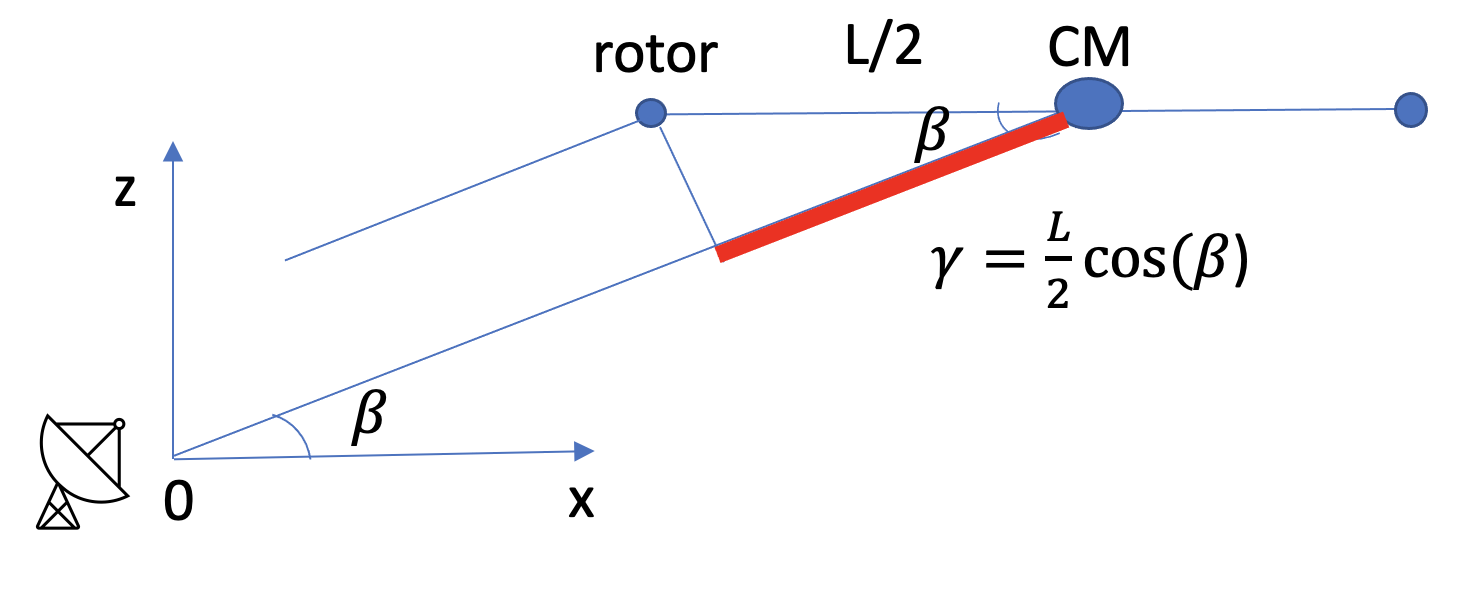
\includegraphics[width=10cm]{FMCW mD analysis-chap4/img/diff_pos_rotors.png}
\caption{Geometric model to determine different positions of rotors}
\label{gemetric_rotors}
\end{figure}

The geometric model just seen is useful for understanding the situation and knowing the maximum values that $\gamma$ can take. Then, to simplify the discussion, it is possible to consider $\gamma$ as a random variable uniformly distributed between its minimum and maximum values.
So the range equation \ref{range_equation_step2} can be rewritten as:
\begin{equation}
R_{point}(t_s,i)=R_{0} + \gamma +(L_1+i \cdot d\rho)\cos \left(\Omega t_{s}+\theta_{0} + k \frac{2\pi}{N_{b}}\right)
\label{step4-range-eq}
\end{equation}

So in the example of quadcopters drones, two rotors are considered at distance $+\gamma$ from $R_{0}$ and the others two are considered at distance $-\gamma$ from $R_{0}$.
To be even closer to reality, it is also possible to consider the different rotational speeds that the different rotors implement during changes of direction or to keep the central body in balance. This can be done by considering the rotation speed of each rotor as a normal random variable with a standard deviation of $10\%$ of its expected value $\Omega$.

Since the equation \ref{step4_formula_model_signal} and \ref{step4-range-eq} were taken into account the presence of $N_{b}$ rotating blades for each $N_{r}$ rotors, which may be at $\gamma$ distance from the centre of mass and which may have a different rotational speed.\\
The last step is to consider also the presence of the central body along with its possible Doppler frequency due to the translatory motion. It's important to consider that because till now we have only considered the rotational motion of the blades. To do that is necessary to sum the \ref{bodycontribution} expression to the \ref{step4_formula_model_signal}.
\begin{equation}
\begin{aligned}
s_{R}(t)=& \sqrt{\sigma_{body}}\operatorname{rect}\left(\frac{t_{f}-2 R_{body}\left(t_{s}\right) / c}{T_{c}}\right) \\
& \cdot \exp \left(j\left(-\frac{4 \pi}{c} \mu t_{f} R_{body}\left(t_{s}\right)-\frac{4 \pi}{c} f_{c} R_{body}\left(t_{s}\right)+\frac{4 \pi \mu}{c^{2}} R_{body}\left(t_{s}\right)^{2}\right)\right)
\end{aligned}
\label{bodycontribution}
\end{equation}

In \ref{bodycontribution} the $\sigma_{body}$ is the RCS body contribution considered as the $25\%$ of the overall drone's RCS. The equation $R_{body}(t_{s})$ now take into account only the presence of the central body at $R_{0}$ distance from radar and its radial velocity $v_{r}$ relative to the radar. The expression is:
\begin{equation}
R_{body}(t_s)=R_{0}+v_{r}t_{s}
\label{range_equation_of body}
\end{equation}

It's important to recall that in all the simulations the drones are considered in hovering state, without any translatory motion in order to emphasize only the rotation motion of the blades.
At the end we obtain the final signal model:

\begin{equation}
\begin{aligned}
&s_{R}(t)=\sqrt{\sigma_{body}}\operatorname{rect}\left(\frac{t_{f}-2 R_{body}\left(t_{s}\right) / c}{T_{c}}\right) \cdot \\
& \exp \left(j\left(-\frac{4 \pi}{c} \mu t_{f} R_{body}\left(t_{s}\right)-\frac{4 \pi}{c} f_{c} R_{body}\left(t_{s}\right)+\frac{4 \pi \mu}{c^{2}} R_{body}\left(t_{s}\right)^{2}\right)\right)+\\
&\sqrt{\frac{\sigma_{blade}}{n_{point} N_b N_r}}\operatorname{rect}\left(\frac{t_{f}-2 R_{point}\left(t_{s},i\right) / c}{T_{c}}\right) \cdot\\
& \sum_{r=1}^{N_{r}} \sum_{k=0}^{N_{b}-1} \sum_{i=1}^{n_{point}} \exp \left(j\left(-\frac{4 \pi}{c} \mu t_{f} R_{point}\left(t_{s},i\right)-\frac{4 \pi}{c} f_{c} R_{point}\left(t_{s},i\right)+\frac{4 \pi \mu}{c^{2}} R_{point}\left(t_{s},i\right)^{2}\right)\right)
\end{aligned}
\end{equation}

It's important to recall that this is the result of the beating between received signal from the target with the reference signal, that is the dechirp operation typically done in FMCW radar and it is not directly the original signal received by the drone. Regarding the step of $\rho$ summations during the simulations the step value of $\rho$ summation was increased linearly until the blade flashes in the analysed planes were well appreciated and the final step chosen is $1.3 cm$, in order to simulate the integral effect. \\
The following table shows the parameters of various drones through which the signals received by them can be simulated using the model shown.

\begin{table}[h!]
\centering
\begin{tabular}{|c|c|c|c|c|c|}
\hline
{\color[HTML]{000000} Model} & {\color[HTML]{000000} $L_1$} & {\color[HTML]{000000} $L_2$} & {\color[HTML]{000000} $\Omega$} & {\color[HTML]{000000} $N_b$} & {\color[HTML]{000000} $N_r$}\\\hline
{\color[HTML]{000000} T-Rex 450} & {\color[HTML]{000000} 42 mm} & {\color[HTML]{000000} 325 mm} & {\color[HTML]{000000} 40 rev/s} & {\color[HTML]{000000} 2} & {\color[HTML]{000000} 1}\\ \hline
{\color[HTML]{000000} T-Rex 500} & {\color[HTML]{000000} 57 mm} & {\color[HTML]{000000} 470 mm} & {\color[HTML]{000000} 46 rev/s} & {\color[HTML]{000000} 2} & {\color[HTML]{000000} 1}\\ \hline
{\color[HTML]{000000} T-Rex 600} & {\color[HTML]{000000} 15 mm} & {\color[HTML]{000000} 600 mm} & {\color[HTML]{000000} 40 rev/s} & {\color[HTML]{000000} 2} & {\color[HTML]{000000} 1}\\ \hline
\end{tabular}
\caption{Helicopter drones model parameters. \cite{align}}
\label{tab:Helicopterdroneparams}
\end{table}

In table \ref{tab:Helicopterdroneparams} helicopter drone parameters to be entered into the model to simulate the signal received from them are shown. 

\begin{table}[h!]
\centering
\begin{tabular}{|c|c|c|c|c|c|l|}
\hline
{\color[HTML]{000000} Model} & {\color[HTML]{000000} $L_1$} & {\color[HTML]{000000} $L_2$} & {\color[HTML]{000000} $\Omega$} & {\color[HTML]{000000} $N_b$} & {\color[HTML]{000000} $N_r$} & Max $\gamma$ \\ \hline
{\color[HTML]{000000} DJI Mavic Air 2} & {\color[HTML]{000000} 5 mm} & {\color[HTML]{000000} 70 mm} & {\color[HTML]{000000} 91.66 rev/s} & {\color[HTML]{000000} 2} & {\color[HTML]{000000} 4} & 91.5 mm \\ \hline
{\color[HTML]{000000} DJI Matrice 300 RTK} & {\color[HTML]{000000} 50 mm} & {\color[HTML]{000000} 266.5 mm} & {\color[HTML]{000000} 70  rev/s} & {\color[HTML]{000000} 2} & {\color[HTML]{000000} 4} & 405 mm \\ \hline
{\color[HTML]{000000} DJI Phantom 4} & {\color[HTML]{000000} 6 mm} & {\color[HTML]{000000} 50 mm} & {\color[HTML]{000000} 116 rev/s} & {\color[HTML]{000000} 2} & {\color[HTML]{000000} 4} & 175 mm \\ \hline
\end{tabular}
\caption{Quadcopter drones parameters.\cite{MartinMulgrew} }
\label{tab:quadcoptersparams}
\end{table}
In table \ref{tab:quadcoptersparams} quadcopter drone parameters to be entered into the model to simulate the signal received from them are shown.

\section{FMCW radar signal processing}
%2D fft signal processing, matrice 3D, implementazione matlab
As initially mentioned at the beginning of the chapter, the choice of use the FMCW radar was preferred over a simple continuous wave radar, in order to be able to perform the analysis in both the Range-Time plane when the migration effect occurs and in the Frequency-Time plane when the migration effect is mitigated. The processing carried out on the signal received from the drone in the case of an FMCW radar is now described. This type of processing is consistent with the received signal model represented in \ref{step4_formula_model_signal}. In fact, it represent the beat signal, i.e. the received signal from drone with the dechirp operation performed on it, which typically occurs in the FMCW radar. The processing performed is commonly referred to as 2DFFT, since two dimensions are measured by this procedure, the distance in range and the speed of the target by means of two successive Fourier transforms. The typical procedure, as described in \cite{2Dprocessing_fmcw}, allows a Range-Time map to be obtained by means of the first Fourier transform, performed for each ramp received from the target. In this map the target is shown in its range bin at the correct distance from the radar. At this point if the migration effect occurs it's possible to appreciate the typical sinusoidal pattern of range changes described in the previous chapter. Then when the range migration is mitigated, by performing a second Fourier transform, this time along the slow time, the Range-Velocity map is obtained. To better understand the procedure just described, a typical example is shown in figure \ref{2dfftimg}.

\begin{figure}[h!]
\centering
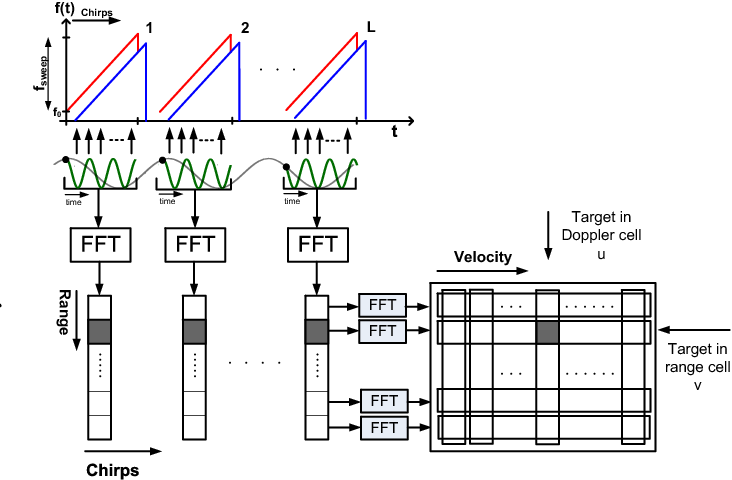
\includegraphics[width=12cm]{FMCW mD analysis-chap4/img/2DFFT radar signal processing.png}
\caption{2DFFT FMCW radar signal processing. \cite{Schroeder2010XbandFR}}
\label{2dfftimg}
\end{figure}

The first part of this procedure is necessary to perform the analysis in the Range-Time plane when the migration effect occurs. On the other hand, for analysis in the Freqeuncy-Time plane when the migration effect does not occur, the second part of this procedure must be modified so that a spectrogram rather than a Range-Doppler map can be obtained. In order to observe a spectrogram, rather than performing the second Fourier transform for all rows of the time-range matrix, it is necessary to perform the Fourier transform for each subset of rows. This is equivalent to performing a Fourier transform every fixed time instant and putting the different results together to obtain the frequency variations occurring during the observation time. Exactly as done for the STFT.\\
So starting from the beginning, the signal received by the radar is 'beaten' with the reference signal and then sampled at the necessary sampling rate to avoid aliasing. 
After being sampled with $f_{ADC} = 2 f_{IFmax}$ we have $M$ samples constituting all the ramps received during the observation time. These $M$ samples are arranged by the radar to form the Chirps-Range Bin matrix. This is a $N_{chirp}$ x $N_{range bin}$ matrix where each row is a chirp and each column is a range bin. Taking the Fourier transform along the Chirps we obtain the Time-Range plane where we expect to observe the target range response. This is possible due to the FMCW radar's characteristic of linking distance to received frequency, so by estimating the frequency of the received signal by means of the FFT, the distance to the target is estimated. Then in order to obtain a spectrogram and analyse the frequency evolution of the target during the observation time, i.e. the duration of each received chirps multiplied for the number of chirps received, we choose a window of length $N_{FFT}$ in which the second Fourier transform is performed. An example is shown in figure \ref{1dmatrix}.

\begin{figure}[h!]
\centering
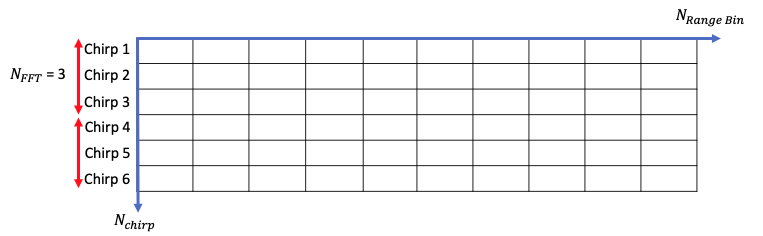
\includegraphics[width=15cm]{FMCW mD analysis-chap4/img/Chirps-Rangebin matrix.png}
\caption{Signal matrix in FMCW radar.}
\label{1dmatrix}
\end{figure}

To better understand we suppose to have only $10$ sample per each received chirp and $6$ chirps. Then the chosen $N_{FFT}$ window length is 3. The second Fourier transform is then performed along the columns, i.e. the range bins. The result of each transformation is a page. In this case as shown in figure \ref{3dmatrix}, we obtain a final $3D$ matrix of dimensions $N_{FFT}$ x $N_{Range bin}$ x $N_{pages}$ where $N_{pages}$ is the number of the total sub Fourier transform. In this case with $6$ received chirps and a window of $N_{FFT} = 3$ we have only 2 pages.

\begin{figure}[h!]
\centering
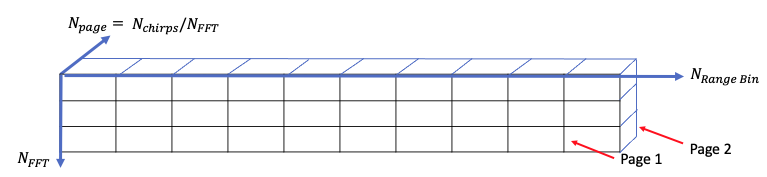
\includegraphics[width=15cm]{FMCW mD analysis-chap4/img/Chirp-rangebin-pages matrix.png}
\caption{Final 3D matrix in FMCW radar processing.}
\label{3dmatrix}
\end{figure}

The last step is to select the range bin in which the target was detected by the first matrix analysis. Extracting all the $N_{pages}$ samples for each chirps yields the desired Frequency-Time matrix corresponding to the spectrogram of the observed target. In figure \ref{finalfreqetimemap} the example is shown where the bin range number 7 is selected and the matrix $N_{FFT}$ x $N_{pages}$ is obtained accordingly. 

\begin{figure}[h!]
\centering
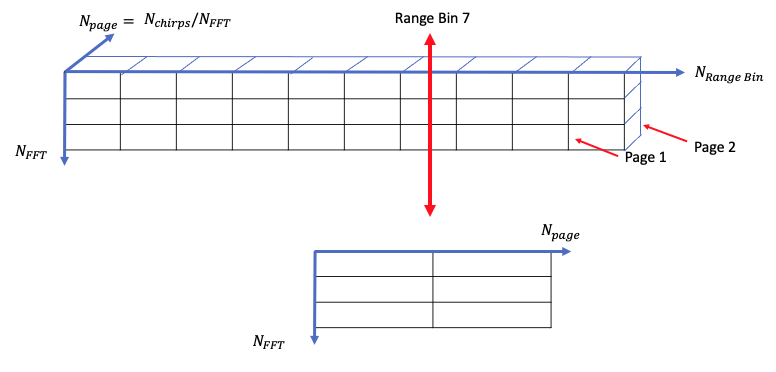
\includegraphics[width=15cm]{FMCW mD analysis-chap4/img/Final frequency time map.png}
\caption{F-t plane in FMCW radar processing.}
\label{finalfreqetimemap}
\end{figure}

This matrix represents the spectrogram of the hypothetical target. It becomes clearly visible why if the cell migration effect occurs, it is not possible to construct the spectrogram of the target due to this processing. In fact, by selecting a range bin, one no longer has all the target information, which would instead be distributed over several range bins. The dimensions and resolutions of the three matrices are now defined:

\begin{itemize}
    \item The starting matrix into which the received signal is inserted;
    
    \item The Time-Range matrix obtained as a result of the first Fourier transform;
         
    \item The Frequency-Time matrix obtained as a result of the second Fourier transform;

\end{itemize}

For the initial matrix of the received signal, each row represents a chirp. Then the y-axis represents time and each time pixel has dimension $T_{chirp}$. Instead, the x-axis represents the number of samples taken with frequency $f_{ADC}$ for the duration of each chirp. Being the frequency related to the distance by the FMCW radar base relation, each pixel has the dimension $dr$. Having sampled the signal at twice the maximum intermediate frequency, in the centre of the matrix there will be the $0$ and in the extremes there will be $-R_{max}$ and $+R_{max}$.\\
The Time-Range matrix, obtained as a result of the first Fourier transform, has the same dimensions as the initial matrix, because by doing the Fourier transform along the rows, the maximum frequency of each ramp and thus the distance of the target is estimated.\\
Finally, the Frequency-Time matrix obtained with performing the second Fourier transform along the columns, shows the frequency along the y-axis. Each pixel in this case represents the frequency resolution, that is the reciprocal of the observation time. Since the signal is observed for $N_{FFT} T_{chirp}$ for each Fourier transform, the frequency resolution will be:
\begin{equation}
\Delta f = \frac{1}{N_{FFT}T_{chirp}}
\end{equation}

Along the x-axis, on the other hand, there is the slow time. The total duration is the number of pages representing the number of sub-transformations performed on the entire signal. While the duration of each page represents the temporal resolution which is:

\begin{equation}
\Delta t = N_{FFT}T_{chirp}
\label{timeres2dfft}
\end{equation}

From the latter expression \ref{timeres2dfft}, it can be seen that compared to the spectrogram constructed by means of the STFT, the temporal resolution is 2 times lower. The main reason for this is due to the fact that the windows with which the different Fourier transforms are carried out do not overlap, as is usually in the case proposed by the STFT. It is possible to implement the oevrlap among windows also in this case as well, it would be necessary to use a window such as the Hamming window, shown in chapter 2. Otherwise, without using any weighting function, the secondary lobes of the sincs due to the windowing lead to blade flashes that still last 2 time pixels. In order to do that each $N_fft$ windows must be shifted of $N_fft/2$ at time and multiplying the signal for the Hamming window before to do the transform. In this way it's possible to achieve a better time resolution as presented in previous section:

\begin{equation}
\Delta t = \frac{N_{FFT}T_{chirp}}{2}
\label{timeresstft}
\end{equation}

\subsection{Simulation example}

Some simulation examples are now shown by performing the processing just described to the signal model already described. First for the drone helicopter and then for the drone quadcopter in the case with and without cell migration. The parameters used for drones are the general ones shown in the table \ref{tab:generaldroneparams}.

\begin{table}[h!]
\centering
\begin{tabular}{|c|c|c|c|c|c|}
\hline
{\color[HTML]{000000} Model} & {\color[HTML]{000000} $L_1$} & {\color[HTML]{000000} $L_2$} & {\color[HTML]{000000} $\Omega$} & {\color[HTML]{000000} $N_b$} & {\color[HTML]{000000} $N_r$} \\ \hline
{\color[HTML]{000000} Helicopter} & {\color[HTML]{000000} 0 mm} & {\color[HTML]{000000} 600 mm} & {\color[HTML]{000000} 25 rev/s} & {\color[HTML]{000000} 2} & {\color[HTML]{000000} 1} \\ \hline
{\color[HTML]{000000} Quadcopter} & {\color[HTML]{000000} 0 mm} & {\color[HTML]{000000} 100 mm} & {\color[HTML]{000000} 100 rev/s} & {\color[HTML]{000000} 2} & {\color[HTML]{000000} 4} \\ \hline
\end{tabular}
\caption{General drones parameters. }
\label{tab:generaldroneparams}
\end{table}

The results that will be shown demonstrate that the signal model used is compatible with other models found in the literature \cite{microdoppler_chen}, \cite{kulpa}. The results also show that the processing performed on the signal to obtain the spectrograms works as expected, in fact the resulted spectrogram are the same as those obtained with the simple STFT.

\subsection{Helicopter drone}
The radar parameters are ideally chosen in order to be able to appreciate the features described. For the case without migration, the duration of the chirp is chosen without considering any constraint, but only respecting the limitation (\ref{chirpmigrationcond}) in order not to incur the migration of the cell. So choosing $T_{chirp} = 70 \mu s$, assuming the drone at distance $R_0 = 0 m$ and assuming the following radar parameters:
\begin{itemize}
    \item $f = 9 GHz$;
    
    \item $\Delta r = 1 m$;
         
    \item $R_{max} = 1000 m$;

    \item $f_{ADC} = 28.5 MHz$;
    
    \item $S = 2141 GHz/s$;
    
    \item $N_{fft} = 22 $;
    
\end{itemize}
Under these conditions we have the following parameters for the Frequency-Time plane: $N_{BF} = 5$, $t_{dwell} = 0.1 s$, $\Delta t = 0.034 s$, $\Delta f = 29.4 Hz$;

In figure \ref{helicrangeprofile} the resulted Range Profile is showed.
It is possible to observe the presence of the target at distance $R_0$ from the radar.

\begin{figure}[h!]
\centering
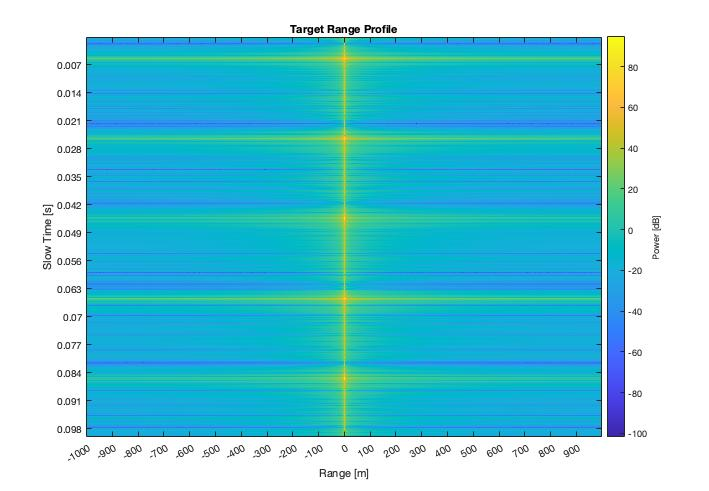
\includegraphics[width=12cm]{FMCW mD analysis-chap4/img/helic_range_profile_example.jpg}
\caption{Helicopter drone range profile.}
\label{helicrangeprofile}
\end{figure}

\begin{figure}[h!]
\centering
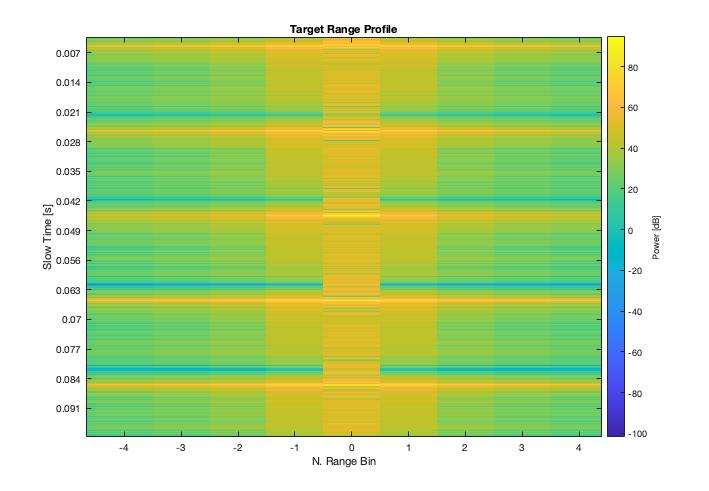
\includegraphics[width=12cm]{FMCW mD analysis-chap4/img/helic_range_bin_example.jpg}
\caption{Helicopter drone range bin visualization.}
\label{helicrangebinprofile}
\end{figure}

In the figure \ref{helicrangebinprofile}, the cells adjacent to the target are zoomed in and it can be observed that with the choice of $T_{chirp}$ made, the cell migration effect does not occur during the observation time.
Continuing the processing and performing the second Fourier transform gives the result shown in figure \ref{helicspectexample}. In order to obtain this result the number of simulating point that compose a blade are linearly increased until we get a fairly clear blade flash. The results shown are simulated considering the presence of 100 points making up a blade, i.e. one point every 6 mm.

\begin{figure}[h!]
\centering
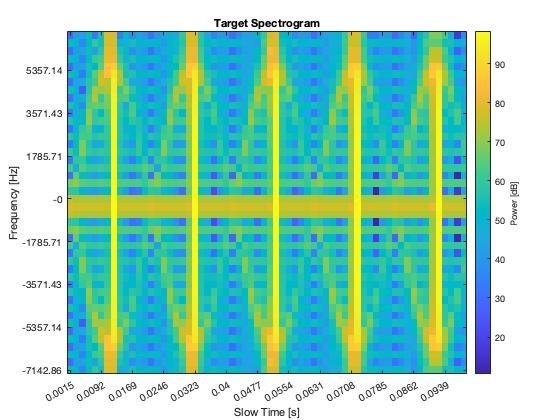
\includegraphics[width=12cm]{FMCW mD analysis-chap4/img/helic_spect_example2.jpg}
\caption{Helicopter drone spectrogram.}
\label{helicspectexample}
\end{figure}

From the result obtained, it is clearly possible to extract visualise the required $N_{BF}$, measure $T_{BF}$ the period between them, the maximum frequency due to the speed of the blade tip $v_{tip}$ and the rotational speed of the rotor $\Omega$.\\
Now the case where the cell migration effect is present is shown, for which a chirp duration is chosen such that the migration condition \ref{chirpmigrationcond} is verified. A chirp is therefore chosen with a duration of $T_{chirp} = 2 ms$. All the radar parameters and target parameteres remains the same as previous except for those that depend on the duration of the chirp:
\begin{itemize}

    \item $f_{ADC} = 1 MHz$;
    
    \item $S = 74.9 GHz/s$;
    
    \item $N_{fft} = 22 $;
    
\end{itemize}
In this case the desired number of blade flash is doubled $N_{BF} = 10$ so also the dwell time is doubled $t_{dwell} = 0.2 s$.
A window of length $N_{fft}$ is also chosen to display what happens in the Freqeuncy-Time plane in the event of migration. Figure \ref{helirangemigr} shows the range profile obtained, where even without zooming in, a characteristic pattern can be seen, similar to that observed in the f-t plane in the case without migration.

\begin{figure}[h!]
\centering
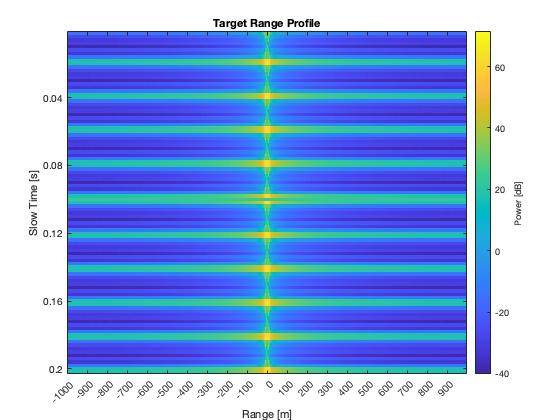
\includegraphics[width=12cm]{FMCW mD analysis-chap4/img/helic_range_migr_example.jpg}
\caption{Helicopter drone Range profile in case of cell migration.}
\label{helirangemigr}
\end{figure}
In the figure \ref{helirangemigrbins}, by zooming in it's possible to clearly observe the range bins over which the target moves during the observation time. As expected theoretically, it is also possible to extract all those features that are extractable on the time-frequency plane, as described in section 1 of this chapter.

\begin{figure}[h!]
\centering
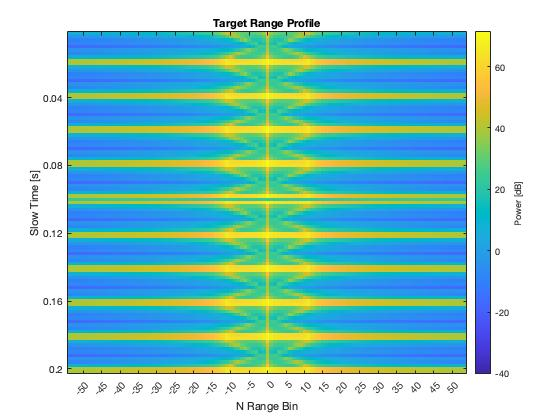
\includegraphics[width=12cm]{FMCW mD analysis-chap4/img/helic_rangebins_migr_example.jpg}
\caption{Helicopter drone Range bins in case of cell migration.}
\label{helirangemigrbins}
\end{figure}

Continuing with the processing and observing the result obtained in the frequency-time plane shows how the migration effect does not make it possible to proceed with classic feature extraction, as the information of the rotating blades changes cell with each chirp received. The result is shown in figure \ref{helirangemigrspect}.

\begin{figure}[h!]
\centering
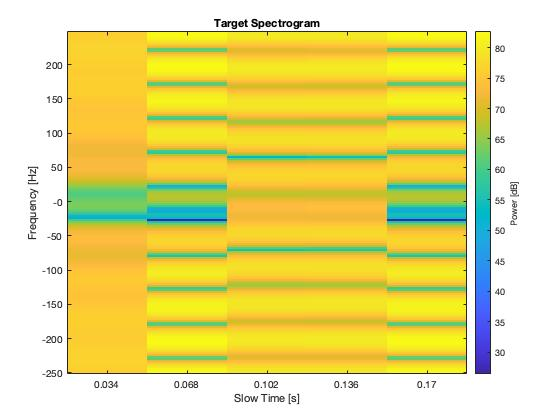
\includegraphics[width=12cm]{FMCW mD analysis-chap4/img/helic_spect_migr_example.jpg}
\caption{Helicopter drone spectrogram in case of cell migration.}
\label{helirangemigrspect}
\end{figure}

However, there are some studies in the literature that use these spectrograms, and by means of a neural network, it is still possible to carry out classification, as shown in \cite{MartinMulgrew}. The spectrogram shown so far have been constructed according to the STFT procedure without overlapping between windows. If we perform the transforms with a $50\%$ overlap between windows and we use a Hamming weighting window, the same spectrograms have a better temporal resolution as shown in the figures \ref{helicspectwithoverlap}.

\begin{figure}[h!]
\centering
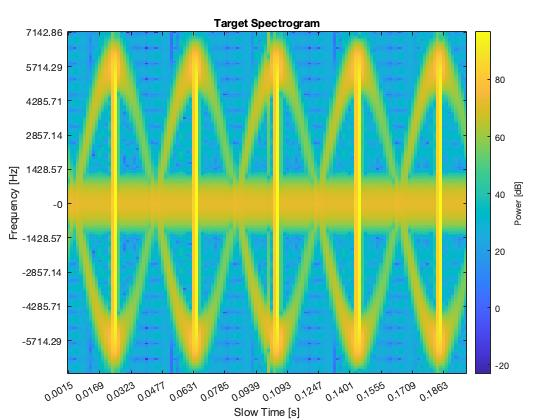
\includegraphics[width=12cm]{FMCW mD analysis-chap4/img/spect_helic_with_overlap.jpg}
\caption{Helicopter drone spectrogram done with overlapping windows.}
\label{helicspectwithoverlap}
\end{figure}

 In this case the temporal resolution is $\Delta t = 0.77 ms$ while in the caso without overlapping time resolution is $\Delta t = 1.5 ms$.
 
\subsection{Quadcopter drone}
Considering the same radar parameters used for the helicopter drone and the same requirements for the time-frequency plane, the spectrogram in the case of a quadcopter drone with charachteristic shown in table \ref{tab:generaldroneparams} is shown in figure \ref{quadspectexample}. In this case by doing the STFT over the column of the Time-Range map is necessary to use the overlapping windows otherwise the time resolution would be too low and would not allow blade flashes to be distinguished between different rotors. 

\begin{figure}[h!]
\centering
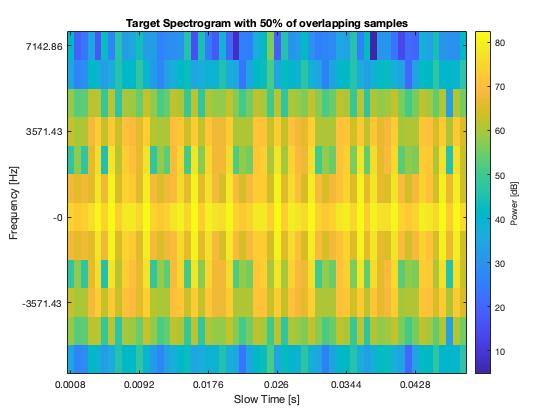
\includegraphics[width=12cm]{FMCW mD analysis-chap4/img/spect_quad_50_perc_overlap.jpg}
\caption{Quadcopter drone spectrogram done with overlapping windows.}
\label{quadspectexample}
\end{figure}

In this case we have set $N_{fft}=12$ while $T_{chirp} = 70\mu s$ is the same as the previous case. Without overlapping among windows in STFT the time resolution is $\Delta t = 0.84 ms$. By setting the overlapping among windows to $50\%$ as explained so far,
the resulted time resolution is $\Delta t = 0.42 ms$, computed as shown in \ref{timeresstft}.

\section{Radar waveform design}
%tenendo in considerazione i limiti e gli obiettivi dei due diversi casi (rho-t e f-t) come deve essere fatta la forma d'onda trasmessa dal radar. Processo di ottimizzazione seguito per massimizzare le risoluzioni (Principalmente durata del chirp e numero di FFT sample per window)
At the beginning of the chapter, we have defined the limitations imposed on the chirp duration and observation time, which are derived from the chosen radar performance parameters and the desired visualisation requirements in the two planes. It is now necessary to understand how to best choose the chirp duration, since as we have seen, everything depends on it. The main objective of the waveform design phase is to determine the chirp duration. The algorithm used to support the decision of the value of $T_{chirp}$ for both Range-Time and Freqeuncy-Time analysis is now described. The main objective is to have the minimum resolution requirements to be met and the minimum number of range or frequency excursions required to be observed. One task of the algorithm is to check whether the minimum resolution requirements can be increased and not only simply satisfy the minimum ones. Using this tool, it is possible to observe which waveform configurations exist that meet the requirements. It will then be necessary to choose the configuration to be used according to the cost-minimisation criterion. The main objective is to check whether there is a single configuration that can meet the requirements of several drone categories or several drone models at the same time. In this way, it would be possible to perform the identification task on several drones with a single waveform.

\subsection{Design for range-time analysis}
Having described the limitations and the requirements present in range-time analysis in section 4.2, the main objective here is to determine $T_{chirp}$ and the others radar parameters in order to have a minimum number of range bins $N_{range-cell}$ migrated from the target at each peak of range variations. Then follows the requirements on the minimum number of range bins $N_{time-cell}$ of duration $\Delta t$ between two maxima of range variations. Finally, it is required to have at least $N_{migr-peak}$, the minimum number of peaks observed in a scan.\\
Each point of the algorithm used to determine the ideal chirp configuration in the case of range-time analysis is now shown:
\begin{itemize}
    \item $1$: Take as input the drone's and radar's parameters;
    
    \item $2$: Take as input the desired observation parameters: $N_{range-cell}$, $N_{time-cell}$ and $N_{migr-peak}$;
         
    \item $3$: Fix $T_{chirp}$ value in order to satisfy all the limitations imposed to it from point 1 and 2 in order to maximize $N_{range-cell}$ and $N_{time-cell}$;

    \item $4$: Check if chosen $T_{chirp}$ value satisfy all the radar constraint;
    
    \item $5$: Give as output the values of all parameters, $\theta_{az}$, $d$, $P_{tx}$, $f_{ADC}$;
    
\end{itemize}
In steps 1 and 2 all the starting parameters of the radar and drone are taken as input, thus we have the constraints on the duration of the chirp forming the two intervals of existence. The first interval is made of all the chirp durations that satisfy the radar constraint, exactly as shown in \ref{radar_limit_interval}. The second interval is made of all the chirp durations that satisfy the desired visualization parameter, as shown in \ref{resolution_limit_interval}. Another limitation from that input data is imposed to dwell time as shown in \ref{dwell_rt_limit}. It is important to consider that in this case, being concerned with migration, the maximum frequency that the radar must be able to measure is the requirement that it must be relaxed, and consequently the only limitation coming from the radar that must be considered is the disambiguity in range.\\
In step 3, the value of $T_{chirp}$ is fixed, taking into account the previous intervals. To try to maximise the requirements, $N_{range-cell}$ and $N_{time-cell}$ are increased by 1 at a time. At each increment, the existence interval of the chirp due to these values is recomputed. The procedure stops when the computed interval of the chirp is no longer compatible with the interval of the chirp due to the radar and drone limitations.\\
in step 5, it is checked that the chosen value is compatible with the range disambiguity requirement.\\
In the last step, all radar parameters that depend on the choice of $T_{chirp}$ are calculated and displayed.
The first parameter $\theta_{az}$, that is the azimuth resolution of the radar, and it is related with the observation time and the renewal time as follow:
\begin{equation}
t_{renew}=\frac{60}{r p m}
\label{renewtime}
\end{equation}
In \ref{renewtime} $rpm$ is the rotation velocity of the antenna and it compare in the expression of the dwell time:

\begin{equation}
t_{d w e l l}=\frac{\theta_{a z}}{6 r p m}
\label{dwelltime}
\end{equation}

We can assume that the minimum dwell time, which depends on $N_{migr-peak}$ that we want to observe, determine the radar azimuth resolution if we consider fixed the renewal time as shown in \ref{thetaz}.

\begin{equation}
\theta_{az}= \frac{t_{dwell} 360}{t_{renew}}
\label{thetaz}
\end{equation}
The azimuth resolution is related also with the antenna dimensions previous denoted as $d$ and with the gain of the antenna as shown in \ref{antennad} and \ref{antennagain}:

\begin{equation}
\theta_{a z}\approx \frac{65 \lambda}{d}
\label{antennad}
\end{equation}

\begin{equation}
G=\frac{4 \pi}{\theta_{a z} \theta_{e l}}
\label{antennagain}
\end{equation}

So as we can understand it is an important parameter and it is useful to minimize it in order to have an higher gain and so a lower transmitted power, a possible way to decrease $\theta_{az}$ is to slow down the speed of antenna rotation.
The required transmit power is calculated by considering the surveillance equation for a continuous wave radar shown in \ref{surveillance_radar_eq}. While the required sampling frequency is calculated from the maximum intermediate frequency received by the target, which therefore depends on the distance at which the object is located and the slope of the radar, as shown in \ref{samplingfreq}. 


\subsection{Design for frequency-time observation}
In this case the objective of the algorithm is to determine $T_{chirp}$ and the others radar parameters in order to have a minimum number of frequency pixels $n_{f}$ at each peak of frequency variations. Then follow the requirements on the minimum number of time pixels $n_{t}$ of duration $\Delta t$ between two blade flashes. Finally, it is required to have at least $N_{BF}$, the minimum number of blade flashes observed in a scan. Each point of the algorithm is now shown:

\begin{itemize}
    \item $1$: Take as input the drone's and radar's parameters and compute the $T_{chirp}$ interval of existence, check that it is consistent;
    
    \item $2$: Take as input the desired observation parameters: $n_{t}$, $n_{f}$ and $N_{BF}$ and compute the relative requirements $\Delta t_{req}$,  $\Delta f_{req}$, $t_{dwell-min}$;
         
    \item $3$: Compute the interval of existence of $N_{fft}$, that contains all possible window lengths of FFTs compatible with the chirp existence interval;

    \item $4$: A $T_{chirp}$ value is fixed for each $N_{fft}$ value, by maximizing $n_{t}$ and $n_{f}$;
    
    \item $5$: For each $N_{fft}$ give as outuput the $T_{chirp}$ choosen value, radar parameters $\theta_{az}$, $d$, $P_{tx}$, $f_{ADC}$ and the obtained resolutions $\Delta t$, $\Delta f$;
    
\end{itemize}

In the first step, as usual, the starting parameters of the radar and the drone parameters are taken as input. The existence interval of $T_{chirp}$ compatible with them is then calculated, as shown in \ref{radar_limit_interval}. In this case, it is important that the radar performs disambiguous measurements in speed. The limitation on chirp duration coming from the maximum frequency can determine a value that is lower than the minimum chirp duration imposed to avoid ambiguity in range measurements. For this reason it is verified that the interval is consistent.\\
In step 2, the required resolutions are computed as shown in \ref{freq-res-ft} and \ref{time_res_req_rt}. Also the minimum dwell time in order to observe $N_{BF}$ is computed.\\
In step 3, since the existence interval of the chirp due to the required resolutions in the f-t plane depends on $N_{fft}$, i.e. the FFT window length, as shown in \ref{res_interval_ft}, the interval of existence of $N_{fft}$ compatible with the first interval of the chirp duration is calculated.\\
In step 4, for each $N_{fft}$ a $T_{chirp}$ value is fixed in order to maximize $n_{t}$ and $n_{f}$, if it is possible. To do that it's possible to increment $n_{t}$ and $n_{f}$ by 1 at time, then the existence interval of chirp due to the newer resolutions is computed. It is check that this interval is compatible with the first interval of chirp due to radar and drone parameters. The procedure stops when the interval of chirp due to resolution is no more compatible with chirp interval due to radar and drone parameters. At the end of the iteration the maximum chirp duration is chosen in order to minimize the slope of the radar and transmitted power.\\
In the last step all the radar parameters for each $N_{fft}$ are displayed, $\theta_{az}$, $d$, $P_{tx}$, $f_{ADC}$, $\Delta t$ and $\Delta f$.


\section{Results}
%risultati ottenuti per i diversi tipi di droni, prima singolarmente poi tabella riassuntiva e infine decisione su come scegliere i parametri per riuscire ad osservere sia i droni quadcopters che helicopters
The algorithms presented are now used with the general parameters of drone helicopter and quadcopter shown in table \ref{tab:generaldroneparams}. These values represent an average of the drone dimensions found in literature as described in \cite{tesiligresti}.
Then the algorithms are also used with the parameters of real drones shown in tables \ref{tab:Helicopterdroneparams} for the helicopter drones and \ref{tab:quadcoptersparams} for the quadcopter drones. 

\subsection{Range-Time analysis results}
\subsubsection{Helicopter drone}
The input radar parameter used are the following:
\begin{itemize}
    
    \item $f=9 GHz$ is the carrier frequency,
         
    \item $\lambda = 0.03 m$ is the wavelength,

    \item $\Delta r = 1 m$ is the resolution in range,
    
    \item $R_{max} = 1000m$ is the maximum range reachable,
    
    \item $B=\frac{c}{2 \Delta r} = 150 MHz$ is the bandwidth,
    
    \item $t_{renew}= 2 \mathrm{~s}$ is the scan time,
    
    \item $SNR = 20 dB$ is the required signal to noise ratio,
    
    \item $\theta_{el}=60^{\circ}$ is the elevation aperture of the beam,
    
    \item $T_{s}=290 \mathrm{~K}$ is the temperature of the system,
    
    \item $F = 10 dB $ is the noise figure of the system.
    
\end{itemize}

 With respect to the typical parameters of state of art's radars the required resolution in range is a little bit relaxed in order to obtain easily realisable slope values and a to obtain a lower sampling frequency.
For the case of generic helicopter drone the parameters are the following:

\begin{itemize}
    
    \item $\Omega = 25*2\pi rad/s$ is the rotation velocity of rotor,
         
    \item $L = 0.6 m$ is the length of blade,

    \item $v_{tip} = 94.25 m/s$ is the blade tip velocity,
    
    \item $N_r = 1$ is the number of rotors,
    
    \item $N_b = 2$ is the number of blades per each rotor,
    
    \item $T_{migr} = \frac{2\pi}{N_b \Omega} = 20 ms$ is the period between two max range variations, 
    
    \item $R_0 = 0m$ is the supposed position of the drone,
    
    \item $\sigma = 0.03 m^{2}$ is the average RCS of a drone helicopter \cite{rcsdrone}.
    
\end{itemize}

The input desired parameters for the range-time analysis are the following:
\begin{itemize}
    
    \item $N_{range-cell} = 5$ is the minimum number required range cells under a peak of range variation,
         
    \item $N_{time-cell} = 5$ is the minimum number required of time cells between two peaks,

    \item $N_{migr-peak} = 5$ is the minimum number of peaks that we want to observe.
    
\end{itemize}

Under this condition the minimum dwell time requested is $T_{dwell} = N_{migr-peak} T_{migr}= 0.1 s$. The resulted value of the azimuth aperture of the beam is $\theta_{az} = 18\degree$. The approximated dimension of the antenna is $d = 0.12m$.\\ Proceeding with the steps of the algorithm described earlier fro the range-time analysis, the iteration of maximization of $N_{range-cell}$ and $N_{time-cell}$ stops with $N_{range-cell} = 10$ and $N_{time-cell} = 10$ and the maximum value of chirp duration chosen is $T_{chirp} = 2 ms$. The minimum value that satisfy the also this resolution requirements is $T_{chirp} = 1.8 ms$. Selecting the maximum value of chirp duration all the others system parameters are the following:

\begin{itemize}
    
    \item $N_{range-cell} = 11$ is the reached number of cell migrated under a peak,
         
    \item $N_{time-cell} = 10$ is the reached number of time cell among two peaks,

    \item $P_{tx} = 81.79 W$ is the necessary transmitted power,
    
    \item $S = 74.9 GHz/s$ is the required chirp slope,
    
    \item $f_{ADC} = 1.01 MHz$ is the required sampling frequency.
    
\end{itemize}

 Investigating the numerical results obtained, the only parameter that could make the analysis difficult is the power required in transmission. In fact, such a high power requirement would make not only the costs too high but a small radar unfeasible. A possible compromise to decrease the power requirement could be to relax the renewal time requirement by accepting that a scan lasts at least 4 seconds. In this case, the azimuth resolution would increase to $9\degree$ and bring the required power to $P_{tx} = 20 W$ that is a feasible result. Another issue could be the required slope, investigating the typical values for chirp generators used in FMCW radars, the state of the art values are around an order of magnitude that is hundreds of tera hertz per second, as explained in \cite{slope}. While as regard the sampling frequency requirement, it can certainly be fulfilled by means of a low-cost solution.\\ By simulating the FMCW radar post processing as described earlier the range time plane obtained is shown in figure \ref{rangetime_map_helic}.

\begin{figure}[h!]
\centering
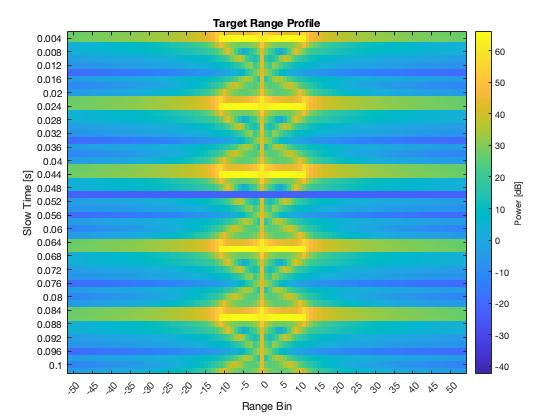
\includegraphics[width=12cm]{FMCW mD analysis-chap4/img/Range-time_generic_helic_result.jpg}
\caption{Range-Time plane of generic helicopter drone.}
\label{rangetime_map_helic}
\end{figure}

 It is clearly possible to extract all the characteristics shown in section 4.2.1, and as in the case of the freqeuncy-time analysis, characteristic blade flashes appear.
 
 \subsubsection{Quadcopter drone}
 
 The results obtained for the quadcopter drone are now shown. Assuming we use the same radar as just shown, the drone input parameters are:
 
 \begin{itemize}
    
    \item $\Omega = 100*2\pi\; rad/s$ is the rotation velocity of rotor,
         
    \item $L = 0.1 m$ is the length of blade,

    \item $v_{tip} = 62.83 m/s$ is the blade tip velocity,
    
    \item $N_r = 4$ is the number of rotors,
    
    \item $N_b = 2$ is the number of blades per each rotor,
    
    \item $T_{migr} = \frac{2\pi}{N_r N_b \Omega} = 1.3 ms$ is the period between two max of the range variations, 
    
    \item $R_0 = 0m$ is the supposed position of the drone,
    
    \item $\sigma = 0.01 m^{2}$ is the average RCS of a drone helicopter \cite{rcsdrone}.
    
\end{itemize}

The input desired parameters are the same as the previous case. Now with $N_{range-cell} = 5 $ and $N_{time-cell} = 5 $ there isn't any interval of chirp duration that satisfy the resolution condition. So we can try relax these requirements by setting $N_{range-cell} = 4 $ and $N_{time-cell} = 4 $. Unfortunately, even in this case it is not possible to meet the resolution requirements, only by accepting $N_{range-cell} = 2 $ and $N_{time-cell} = 2 $ there is a compatible value of $T_{chirp} = 0.625ms$. Under this condition the minimum dwell time requested is $t_{dwell} = N_{migr-peak} T_{migr}= 6.3 ms$, that is much lower than that required for an helicopter drone. The result value of the azimuth aperture of the beam is $\theta_{az} = 1.25\degree$. Follow that the approximated dimension of the antenna begins to be too big and incompatible with the need for small dimension, it is $d = 1.9m$. It's possible to decrease it by increasing the observation time, considering that we want to observe 5 peaks of migration that belongs to the same rotor and not 5 peaks of migration that belongs to any rotors. We obtain $t_{dwell} = N_{migr-peak} T_{migr}= 25 ms$. The value of azimuth aperture increase to $\theta_{az} = 4.5\degree$ and led to an antenna dimension of $d = 0.48m$, that is feasible. But just 2 pixels between two blade flashes still does not permit to distinguish the number of rotors, as shown in figure \ref{rangetime_map_quad_4rot}. In addition the migration of only two range cells in real scenario may not always be detected. It is therefore decided to consider the period between two blade flashes of the same rotor as a design parameter.  Now the optimisation phase produce a max resolution values of $N_{range-cell} = 4$ and $N_{time-cell} = 4$. The minimum value that satisfy the resolution requirements is $T_{chirp} = 1.1 ms$ while the maximum one is $T_{chirp} = 1.3 ms$. As usual we choose the maximum one.
With this value of chirp duration all the others system parameters are the following:

\begin{itemize}
    
    \item $N_{range-cell} = 5$ is the reached number of cell migrated under a peak,
         
    \item $N_{time-cell} = 4$ is the reached number of time cell among two peaks,

    \item $P_{tx} = 17 W$ is the necessary transmitted power,
    
    \item $S = 119.9 GHz/s$ is the required chirp slope,
    
    \item $f_{ADC} = 1.6 MHz$ is the required sampling frequency.
    
\end{itemize}

In this case, the required power has an acceptable value, this is due to the fact that azimuth aperture is very low and led to an high gain of the antenna. The result obtained by simulating FMCW radar processing is shown in figure \ref{rangetime_map_quad}.

\begin{figure}[h!]
\centering
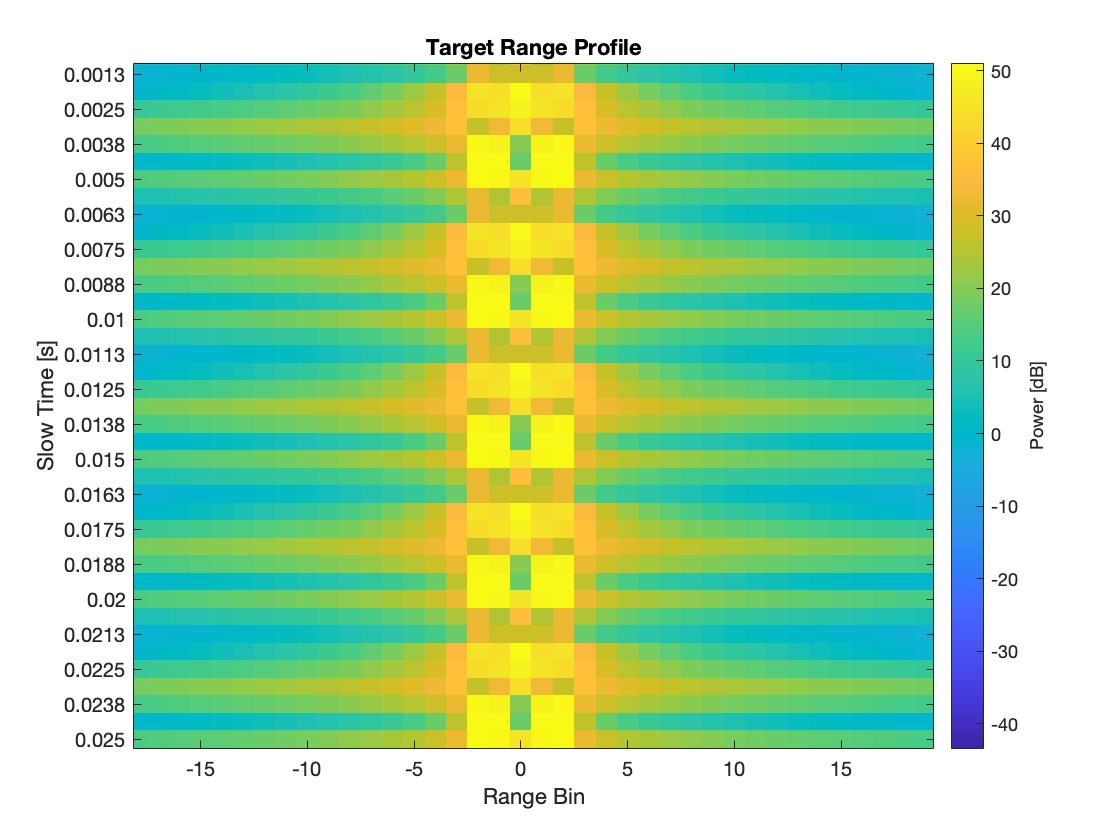
\includegraphics[width=10cm]{FMCW mD analysis-chap4/img/quad_range_var_no_good.jpg}
\caption{Range-Time plane of quadcopter drone built with $T_{BF}$ of 4 rotors.}
\label{rangetime_map_quad_4rot}
\end{figure}

\begin{figure}[h!]
\centering
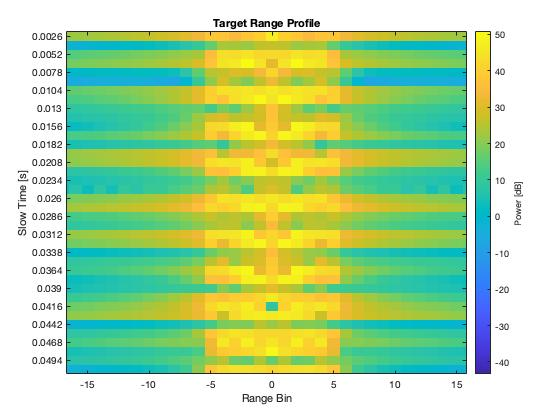
\includegraphics[width=10cm]{FMCW mD analysis-chap4/img/quadcopter_range_profile.jpg}
\caption{Range-Time plane of quadcopter drone built with $T_{BF}$ of 1 rotors.}
\label{rangetime_map_quad}
\end{figure}

In this case, considering that each rotor has a different initial random phase, it is possible to extract the period information between two blade flashes of the same rotor only when the positions of the blade flashes are not such that a continuous band. In this unfortunate case, it is still possible to extract the migrated cell information that leads to the product blade length per rotation rate that is the blade tip velocity information.\\
Summarising the results obtained for the range-time analysis, giving the same importance to the frequency and time resolution, it is always feasible to extract the information for a generic helicopter drone in a comprehensive manner. For a generic quadcopter drone, on the other hand, it is only possible to extract all the information when the conditions of the initial phase of the different rotors allow it, i.e. the blade flashes are not arranged in such a way as to form a continuous band, or they overlap. In this case using a $T_{chirp} = 0.625ms$ it is always possible to extract the information on blade length and rotation speed, while it is only possible to extract the information about the number of rotors only when the initial phase conditions allow it. At the end with this chirp duration the migrated cell in a peak of migration are only 2.\\
Increasing the duration of the chirp to $T_{chirp} = 1.3ms$ makes the extraction of the rotational speed information dependent on the initial phase of the different rotors, since as explained so far in some conditions a continuous band could be observed. On the other hand, with this configuration it's possible to have 5 migrated cells. So in lucky case it's possible to extract all the drone's features except the number of rotors. While, if we use the lower chirp duration, in lucky case it's possible to extract all the drone's features, also the number of rotors.

\subsubsection{Unique waveform}

Trying to find a unique waveform that allows the information of both a quadcopter and a helicopter drones to be extracted, the experiments performed show that it is clearly possible to extract all the information of a helicopter drone even with a chirp duration $T_{chirp} = 0.625 ms$. Considering that the range resolution of the radar is $1 m$, it could be considered acceptable to have a migration of only two cells for a quadcopter drone. The required observation time should be the longer one needed for the helicopter drone: $t_{dwell} = 0.1s$.
Considering the longer observation time and the lower chirp duration these led to a very high power requirement of $P_{tx} = 785 W$ in case of quadcopter drone that has the lower RCS. Also by increasing the scan time to 4 second the necessary power is always $P_{tx} = 196 W$. So we must relax the chirp duration or the maximum range distance at which we would recognize a quadcopter, or the number of subsequent peaks that we would observe. If we accept to not extract the information about the number of rotors, we can set $T_{chirp} = 1.3ms$. In this case the required transmitted power is $P_{tx} = 94.3 W$ with scan time of 4 seconds. If we increments this parameter to 6 seconds we obtain $P_{tx} = 41.9 W$.
Summarizing the radar parameters with this choice are:
\begin{itemize}

    \item $T_{chirp} = 1.3ms$ is the chirp duration,
    
    \item $t_{dwell} = 0.1s$ is the observation time,
    
    \item $t_{srenew} = 6 s$ is the scan time,

    \item $d = 0.24 m$ is the required antenna dimension,
         
    \item $\theta_{az} = 9\degree$ is the required azimuth resolution,

    \item $P_{tx} = 41.9 W$ is the necessary transmitted power,
    
    \item $S = 115.3 GHz/s$ is the required chirp slope,
    
    \item $f_{ADC} = 1.54 MHz$ is the required sampling frequency.
    
\end{itemize}
In the following figures \ref{helic_unique_waveform} and \ref{quad_unique_waveform} the result obtained for the helicpoter and the quadcopter drone observed with the same waveform are shown.

\begin{figure}[h!]
\centering
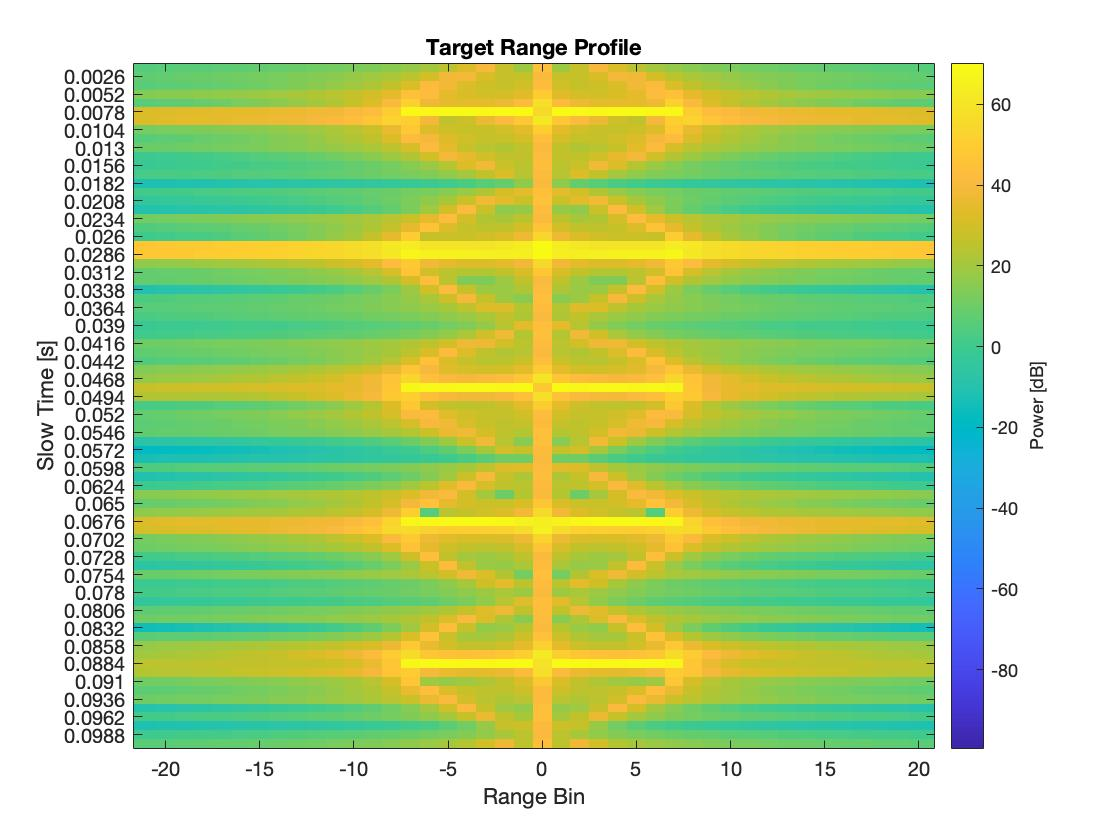
\includegraphics[width=10cm]{FMCW mD analysis-chap4/img/range-time_helic_with_unique_wavform.jpg}
\caption{Range-Time plane of helicopter drone observed with waveform compatible with quadcopter drone.}
\label{helic_unique_waveform}
\end{figure}

\begin{figure}[h!]
\centering
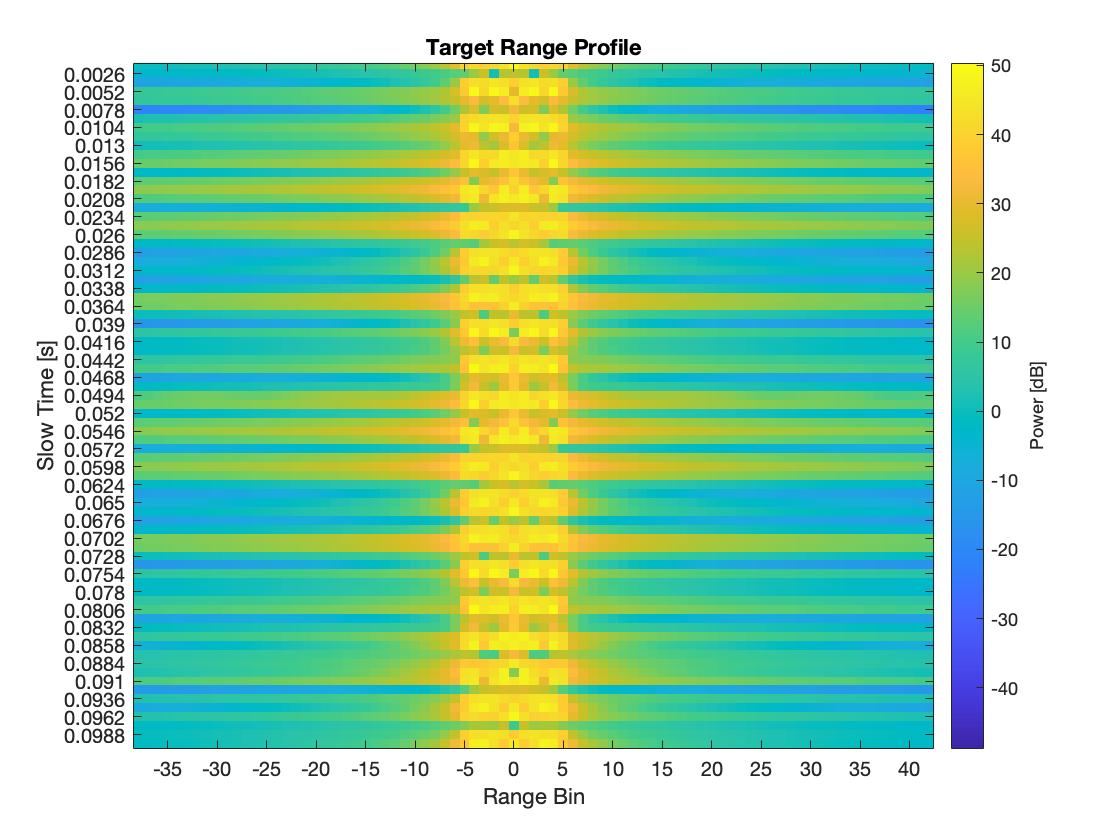
\includegraphics[width=10cm]{FMCW mD analysis-chap4/img/range-time_quaad_unique_wave.jpg}
\caption{Range-Time plane of quadcopter drone observed with waveform compatible with helicopter drone.}
\label{quad_unique_waveform}
\end{figure}

As can be seen it's possible to extract all the features from the helicopter range profile, the length of the blade $L$, the rotation rate of the rotor $\Omega$ and the number of blades $N_b$. In this fortunate case, it's possible to extract the following features from the quadcopter range profile: the length of the blade $L$, the rotation rate of the rotor $\Omega$, the number of blades $N_b$. The only information that is not possible to extract is the number of rotors. In unfortunate case the different initial phase of rotor doesn't allow to extract also the information of rotation rate of the rotor. But it' always possible to extract the the product $L\Omega$ that is the blade tip velocity and it can be a very useful information for the classification task. 

\subsection{Freqeuncy-Time analysis results}
\subsubsection{Helicopter drone}

The input radar parameter used are the same as for the range-time analysis, also the input parameters of the generic helicopter drone are the same with the only change in the notation for the period between 2 blade flashes, instead of $T_{migr}$, now it's called $T_{BF}$.\\
Now the input desired parameters for the frequency-time analysis are the following:
\begin{itemize}
    
    \item $n_{t} = 5$ is the minimum number of time pixels required between 2 blade flashes,
         
    \item $n_{f} = 5$ is the minimum number of frequency pixel required between 2 blade flashes,

    \item $N_{BF} = 5$ is the minimum number of blade flashes that we want to observe.
    
\end{itemize}

Under this condition the minimum dwell time requested is $t_{dwell} = N_{BF} T_{BF}= 0.1 s$. The resulted value of the azimuth aperture of the beam is $\theta_{az} = 18\degree$. The approximated dimension of the antenna is $d = 0.12m$.\\ Proceeding with the steps of the algorithm described earlier for the frequency-time analysis, the interval of existence of $N_{fft}$, i.e the FFT window length, is between $N_{fft} = 10$ and $N_{fft} = 120$. For each $N_{fft}$ value the maximum possible chirp duration that respect all the radar constraint is chosen and all the others radar parameters are computed. In table \ref{tab:fthelicresult} are reported the results.
\begin{table}[h!]
\centering
\begin{tabular}{|c|c|c|c|c|c|c|}
\hline
$N_{fft}$ & $T_{chirp}$ & $\Delta f$ & \begin{tabular}[c]{@{}c@{}}$\Delta t$\end{tabular} & $P_{tx}$ & $S$ & $f_{ADC}$ \\ \hline
12 & 88.35 $\mu$s & 943.13 Hz & 0.53 ms & 154.2W & 1696 GHz/s & 22.6 MHz \\ \hline
20 & 88.35 $\mu$s & 565.88 Hz & 0.88 ms & 92.5 W & 1696 GHz/s & 22.6 MHz \\ \hline
28 & 88.35 $\mu$s & 404.19 Hz & 1.23 ms & 66.12 W & 1696 GHz/s & 22.6 MHz \\ \hline
34 & 78.43 $\mu$s & 375 Hz & 1.33 ms & 61.34 W & 1911 GHz/s & 25.5 MHz \\ \hline
42 & 68.02 $\mu$s & 350 Hz & 1.42 ms & 57.2 W & 2203 GHz/s & 29.4 MHz \\ \hline
50 & 72.72 $\mu$s & 275 Hz & 1.81 ms & 44.9 W & 2061 GHz/s & 27.5 MHz \\ \hline
58 & 68.9 $\mu$s & 250 Hz & 2 ms & 40.8 W & 2173 GHz/s & 29 MHz \\ \hline
\end{tabular}
\caption{Radar parmeters results for each $N_{fft}$ chosen value for the generic helicopter drone with a $t_{renew} = 2s$ and $t_{dwell} = 0.1s$.}
\label{tab:fthelicresult}
\end{table}

The only parameter that could be unfeasible is the required transmission power, which as seen decreases with increasing the FFT window length because the number of ramps that can be coherently integrated increases. The values obtained were calculated by setting the scan time at 2 seconds. As done in the range-time analysis, it is possible to decrease the antenna rotation speed and thus increase the renewal time to 4 or 6 seconds in order to obtain feasible values of transmitted power. Taking for example the $N_{fft}=42$, and increasing the renewal time to 4 seconds the azimuth aperture of the beam became $\theta_{az} = 9\degree$. The approximated dimension of the antenna is $d = 0.24m$. The necessary trasmitted power became $P_{tx} = 14.31 W$. The post-processing FMCW radar result are shown in figure \ref{generic_f-t_helic}.

\begin{figure}[h!]
\centering
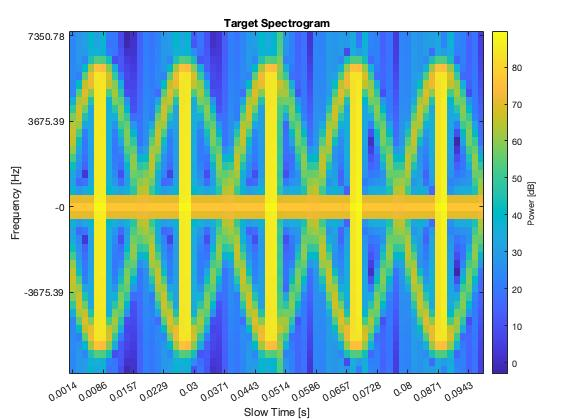
\includegraphics[width=12cm]{FMCW mD analysis-chap4/img/helic_spect_f-t_dimension.jpg}
\caption{Frequency-Time plane of generic helicopter.}
\label{generic_f-t_helic}
\end{figure}

In this case, it is easy to extract all the features of the observed helicopter drone without any problems, the length of the blade $L$, the rotation rate of the rotor $\Omega$ and the number of blades $N_b$.\\

\subsubsection{Quadcopter drone}
Considering now the case of the generic quadcopter drone, assuming that we always use the same radar with the same initial parameters, the drone parameters are the same as in the case of range-time analysis. Also now if we consider $T_{BF} = \frac{2\pi}{N_r N_b \Omega} = 1.3 ms$ as the period between two consecutive blade flash of any rotor, no solution can be found that meets the resolution requirements. So we consider the period between two blade flashes to be that of the same rotor $T_{BF} = \frac{2\pi}{N_b \Omega} = 5 ms$. 
Considering the same visualization requirements as for the drone quadcopter: 
\begin{itemize}
    
    \item $n_{t} = 5$ is the minimum number of time pixels required between 2 blade flashes,
         
    \item $n_{f} = 5$ is the minimum number of frequency pixel required between 2 blade flashes,

    \item $N_{BF} = 5$ is the minimum number of blade flashes that we want to observe.
    
\end{itemize}

The blade flash period for the single rotor of the generic quadcopter drone is $T_{BF} = 5 ms$, with the renewal timw $t_{renew} = 2 s$ and the minimum dwell time is $t_{dwell} = 25 ms$ and we obtain the beam azimuth aperture $\theta_{az} = 4.5\degree$. The the antenna dimension is $d = 0.48m$.\\
Proceeding with the next steps of the algorithm, we obtain that the values of FFT window length ranging from $N_{fft} = 10$ up to $N_{fft}= 28$ satisfy the resolution requirements. The relative radar parameters are given in table \ref{tab:ftquadresult}.

\begin{table}[h!]
\centering
\begin{tabular}{|c|c|c|c|c|c|c|}
\hline
$N_{fft}$ & $T_{chirp}$ & $\Delta f$ & $\Delta t$ & $P_{tx}$ & $S$ & $f_{ADC}$ \\ \hline
12 & 132.53 $\mu$ s & 628.7 Hz & 0.79 ms & 19.28 W & 1130 GHz/s & 15.09 MHz \\ \hline
16 & 99.40 $\mu$s & 628.7 Hz & 0.79 ms & 19.28 W & 1507 GHz/s & 20.12 MHz \\ \hline
20 & 79.52 $\mu$s & 628 Hz & 0.79 ms & 19.28 W & 1884 GHz/s & 25.17 MHz \\ \hline
24 & 66.7 $\mu$s & 624 Hz & 0.80 ms & 19.28 W & 2246 GHz/s & 29.9 MHz \\ \hline
28 & 66.7 $\mu$s & 535 Hz & 0.93  ms & 16.4 W & 2246 GHz/s & 29.9 MHz \\ \hline
\end{tabular}
\caption{Radar parameter results for each $N_{fft}$ chosen value for the generic quadcopter drone  with a $t_{renew} = 2s$ and $t_{dwell} = 25ms$.}
\label{tab:ftquadresult}
\end{table}

In this case, more weight was given to temporal resolution by choosing the chirp with the minimum duration that satisfy both the resolution and the radar requirements for each $N_{fft}$. 
As usual, if we need to decrease the required transmission power, we can decrease the antenna rotation speed until a renewal time of 4 to 6 seconds is achieved. As for the slope parameter required for the chirp, it is higher in this case due to the shorter chirp duration. As mentioned for the range-time analysis case, these values are within the hundreds of $THz$ per second limits of the state of the art.
On the basis of the simulations carried out, it is clear that it is necessary to increase the frequency resolution in order to be able to correctly extract all the information from the quadcopter spectrogram. If we accepts to have only 3 frequency pixels below a peak, using the minimum chirp duration imposed by the range disambiguity $T_{chirp} = 66.7 \mu s$ and $N_{fft} = 12$ it's possible obtain 12 temporal pixels between two blade flash of the same rotor. Under this condition the following radar parameters are:

\begin{itemize}
    
    \item $\Delta f = 1249 Hz$ is the achieved frequency resolution,
    
    \item $\Delta t = 0.4 ms$ is the achieved time resolution,
    
    \item $d = 0.48 m$ is the required antenna dimension,
         
    \item $\theta_{az} = 4.5\degree$ is the required azimuth resolution,

    \item $P_{tx} = 38.32 W$ is the necessary transmitted power,
    
    \item $S = 2246 GHz/s$ is the required chirp slope,
    
    \item $f_{ADC} = 29.9 MHz$ is the required sampling frequency.
    
\end{itemize}

Figures \ref{generic_f-t_helic} show the results obtained following 2DFFT processing of the FMCW radar in the case where the spectrogram is constructed with $50\%$ overlapping of windows and in the figure \ref{generic_f-t_quad} with $75\%$ overlapping of windows. In this last case the time resolution achieved is $\Delta t = 0.2 ms$, two time better than the case of $50\%$ of overlapping. 

\begin{figure}[h!]
\centering
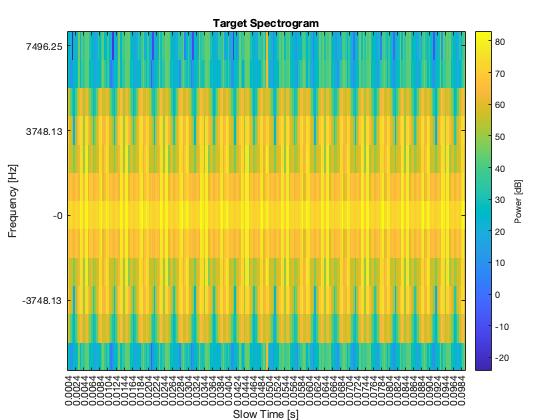
\includegraphics[width=12cm]{FMCW mD analysis-chap4/img/quad_spect_max_res_50.jpg}
\caption{Spectrogram of quadcopter built with $50\%$ of overlapping windows.}
\label{generic_f-t_helic}
\end{figure}

\begin{figure}[h!]
\centering
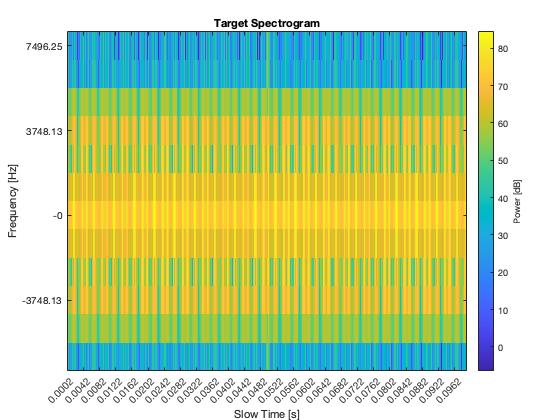
\includegraphics[width=12cm]{FMCW mD analysis-chap4/img/quad_spect_max_res_75.jpg}
\caption{Spectrogram of quadcopter built with $75\%$ of overlapping windows.}
\label{generic_f-t_quad}
\end{figure}

Under these conditions, it is possible to extract all the necessary information from the spectrograms, the length of the blade $L$, the rotation rate of the rotor $\Omega$, the number of blades $N_b$ and the number of rotor $N_r$ in the lucky case that the initial phase differences of the different rotors allow this. With the overlapping set to $75\%$ it is more likely to be able to measure the number of rotors present regardless of their initial phase difference, as there are twice time pixels between two blade flashes belonging to the same rotor with respect to the case of $50\%$ of overlapping.\\

\subsubsection{Unique waveform}
Since we are interested in finding a single waveform that will allow us to extract the features of both helicopter drone and quadcopter drone, the observation time required is the longest ones coming from the helicopter drone $t_{dwell} = 0.1s$, while the time resolution needed is the ones of quadcopter which has the lower blade flash period. So by we set the chirp duration to $T_{chirp} = 66.7 \mu s$ and the length of FFT window to $N_{fft} = 12$. Under these condition, with the renewal time $t_{renew} = 2s$ the necessary transmitted power for a quadcopter drone is $P_{tx} = 613 W$. In order to decrease this value, we can try to relax the renewal time to $6 s$ and the number of required blade flash to $4$. In this way the dwell time decrease by $20 ms$ and become $t_{dwell} = 0.08 s$. The beam azimuth aperture become $\theta_{az} = 4.8\degree$. The final required transmitted power is $P_{tx} = 43.6 W$. That is also an high value, and decreasing the renewal time so much is not one of the best choices. At this point, the most convenient choice might be to decrease the coverage range for small quadcopter drones only. Decreasing the identification range from $1000 m$ to $800 m$ results in a required transmitted power of $P_{tx} = 17.8 W$. So at the end the resulted parameters are:

\begin{itemize}
    
    \item $T_{chirp} = 66.7 \mu s$ is the chirp duration,
    
    \item $\Delta f = 1249 Hz$ is the achieved frequency resolution,
    
    \item $\Delta t = 0.4 ms$ is the achieved time resolution,
    
    \item $d = 0.45 m$ is the required antenna dimension,
         
    \item $\theta_{az} = 4.8\degree$ is the required azimuth resolution,

    \item $P_{tx} = 17.8 W$ is the necessary transmitted power,
    
    \item $S = 2247 GHz/s$ is the required chirp slope,
    
    \item $f_{ADC} = 30 MHz$ is the required sampling frequency,
    
    \item $R_{max} = 800 m$ is the maximum identification range for a quadcopter drone.
    
    \item $R_{max} = 1000 m$ is the maximum identification range for a helicopter drone

    
\end{itemize}

In figure \ref{generic_f-t_helic_unique} and \ref{generic_f-t_quad_unique} are shown the simulation result of post-processing done with the FMCW radar, in this case the overalapping among FFT window is set to $75\%$, in this way the theoretical resolution in time would be $0.2ms$.

\begin{figure}[h!]
\centering
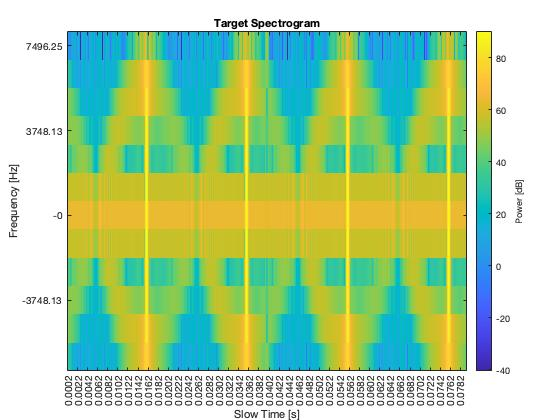
\includegraphics[width=12cm]{FMCW mD analysis-chap4/img/helic_unique_ft.jpg}
\caption{Spectrogram of generic helicopter observed with unique waveform.}
\label{generic_f-t_helic_unique}
\end{figure}

\begin{figure}[h!]
\centering
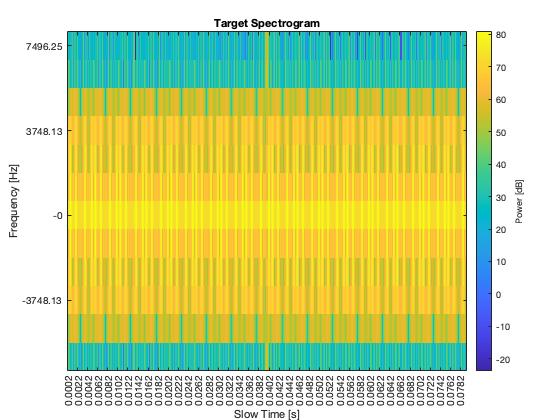
\includegraphics[width=12cm]{FMCW mD analysis-chap4/img/quad_unique_wave_ft.jpg}
\caption{Spectrogram of generic quadcopter observed with unique waveform.}
\label{generic_f-t_quad_unique}
\end{figure}

As can be seen from the figures just shown, it is clearly possible to extract all features in the case of both the helicopter drone and the quadcopter drone. But in order to achieve this result, much more importance has been attached to the temporal resolution, one could think that a frequency resolution of $\Delta f = 1249 Hz$ might not be sufficient. In order to try to balance a little bit the resolutions we can try to increase the chirp duration. If we accepts that it is not always possible to discriminate the number of different rotors, but only in cases where the phase difference between them allows it, it is possible to increase the duration of the chirp to $T_{chirp} = 80 \mu s$ in order to gain some frequency resolution. Thus we obtain $\Delta t = 0.24 ms$ in the case of overlap between the windows at $75\%$ and $\Delta f = 1041 Hz$. By further increasing the chirp duration, the assumption of being able to measure the number of rotors present must be abandoned.

\subsection{Result with different drones}

The analysis is now carried out on the drones model shown in tables  \ref{tab:Helicopterdroneparams} and \ref{tab:quadcoptersparams}.
First the result obtained with the waveform design algorithm are presented. Then the unique waveform obtained in the previous section is applied and and the results are shown.

\subsubsection{Range-time analysis}
In the table \ref{tab:rt-helic-result}  is shown the result of waveform design algorithm applied to the three helicopter drones T-Rex 450, T-Rex 500 and T-Rex 600. The scan time is set to $t_{renew} = 2s$. 
\begin{table}[h!]
\centering
\begin{tabular}{|c|c|c|c|c|c|c|c|}
\hline
$T_{chirp}$ & $N_{range-cell}$ & $N_{time-cell}$ & $P_{tx}$ & S & $f_{ADC}$ & $t_{dwell}$ & $\theta_{az}$ \\ \hline
1.8 ms & 7 & 7 & 35.7 W & 83.9 GHz/s & 1.12 MHz & 62.5 ms & 11.25$\degree$ \\ \hline
1.2 ms & 9 & 9 & 40 W & 124 GHz/s & 1.67 MHz & 54 ms & 9.78$\degree$ \\ \hline
1.3 ms & 10 & 10 & 51.12 W & 119 GHz/s & 1.61 MHz & 62.5 m & 11.25$\degree$ \\ \hline
\end{tabular}
\caption{Radar parameters result for r-t analysis for the T-Rex 450, T-Rex 500 and T-Rex 600 drones.}
\label{tab:rt-helic-result}
\end{table}
Applying the unique waveform designed in the previous section for the range-time analysis, the following characteristics and all the other radar parameters are:
\begin{itemize}

    \item $T_{chirp} = 1.3ms$ is the chirp duration,
    
    \item $t_{dwell} = 0.1s$ is the observation time,
    
    \item $t_{renew} = 6 s$ is the scan time,

    \item $d = 0.36 m$ is the required antenna dimension,
         
    \item $\theta_{az} = 6\degree$ is the required azimuth resolution,

    \item $P_{tx} = 13.98 W$ is the necessary transmitted power,
    
    \item $S = 115.3 GHz/s$ is the required chirp slope,
    
    \item $f_{ADC} = 1.54 MHz$ is the required sampling frequency.
    
\end{itemize}
By using this configurations the result obtained for the three helicopter drone described in \ref{tab:Helicopterdroneparams} clearly show the characteristics to be extracted.

\begin{figure}[h!]
\centering
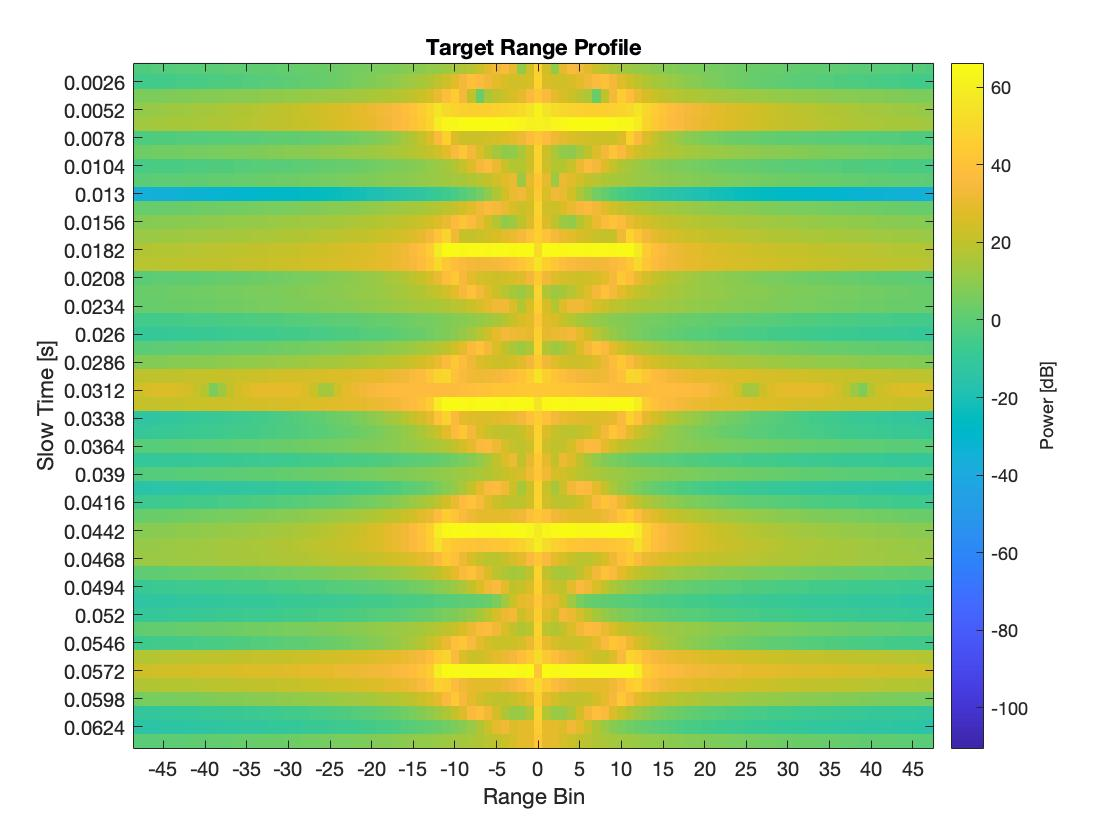
\includegraphics[width=9cm]{FMCW mD analysis-chap4/img/t-rex-600-rt-unique.jpg}
\caption{Range profile of T-Rex 600 observed with unique waveform.}
\label{t-rex600-unique-wave-rt}
\end{figure}

As an example, the range profile obtained for the T-Rex 600 drone is shown in figure \ref{t-rex600-unique-wave-rt}, from which all possible classification information can be extracted. The measured distance between two blade flashes is 10 pixels, resulting in a measured period of $T_{migr} = 0.0130s$ compared to the actual value of $T_{migr} = 0.0125s$. The measured range pixels on a blade flash are 11, corresponding to a migration $R_{migr}=11m$ from which we obtain a maximum blade tip speed of $v_{tip} = 128.1164 m/s$. The  number of blades extracted is $N_b = 2$ and by adding to it the knowledge of $T_{BF}$ the resulting rotation rate measured is $\Omega = 241.66 rad/s$. The resulting blade length measured is $L = 0.58 m$ while the real blade length is $ L = 0.6 m$. \\
For the T-Rex 450 model the measured distance between two blade flashes is 10 pixels, resulting in a measured period of $T_{migr} = 0.0130s$ compared to the actual value of $T_{migr} = 0.0125s$. The measured range pixels on a blade flash are 6, corresponding to a migration $R_{migr}=6m$ from which we obtain a maximum blade tip speed of $v_{tip} = 76.86 m/s$. The  number of blades extracted is $N_b = 2$ and by adding to it the knowledge of $T_{BF}$ the resulting rotation rate measured is $\Omega = 241.66 rad/s$. The resulting blade length measured is $L = 0.318 m$ while the real blade length is $ L = 0.325 m$.\\
Making the same procedure for the last, T-Rex 500 model, For the T-Rex 450 model the measured distance between two blade flashes is 10 pixels, resulting in a measured period of $T_{migr} = 0.0104s$ compared to the actual value of $T_{migr} = 0.0109s$. The measured range pixels on a blade flash are 11, corresponding to a migration $R_{migr}=11m$ from which we obtain a maximum blade tip speed of $v_{tip} = 140.92 ms$. The  number of blades extracted is $N_b = 2$ and by adding to it the knowledge of $T_{BF}$ the resulting rotation rate measured is $\Omega = 302.07 rad/s$. The resulting blade length measured is $L = 0.46 m$ while the real blade length is $ L = 0.47 m$.\\
The results obtained by applying the waveform design algorithm to the DJI Mavic Air 2, DJI Matrice 300 and DJI Panthom 4 drones give the configurations shown in the table \ref{tab:rt-quad-result}. The scan time is set to $t_{renew} = 2s$.
\begin{table}[h!]
\centering
\begin{tabular}{|c|c|c|c|c|c|c|c|}
\hline
$T_{chirp}$ & $N_{migrazione-cell}$ & $N_{time-cell}$ & $P_{tx}$ & S & $f_{ADC}$ & $t_{dwell}$ & $\theta_{az}$ \\ \hline
1.8 ms & 3 & 3 & 20 W & 82.3 GHz/s & 1.1 MHz & 27.3 ms & 4.9$\degree$ \\ \hline
1 ms & 7 & 7 & 61 W & 146.8 GHz/s & 1.97 MHz & 35.7 ms & 6.42$\degree$ \\ \hline
1.4 ms & 3 & 3 & 15.8 W & 104.3 GHz/s & 1.39 MHz & 21.6 m & 3.87$\degree$ \\ \hline
\end{tabular}
\caption{Radar parameters result for range-time analysis for the DJI Mavic Air 2, DJI Matrice 300, and DJI Panthom 4 drones.}
\label{tab:rt-quad-result}
\end{table}
Applying the unique waveform described earlier now the only value that changes is the power required in transmission due to the lower RCS of quadcopter drones, that is $P_{tx} = 41.94 W$. As we have already seen, in the case of quadcopters, this requirement can be greatly reduced by decreasing the maximum classification range to $800m$, in which case the required power becomes $P_{tx} = 17.18W$.
As an example, the range profile obtained for the DJI Mavic Air 2 drone is shown in figure \ref{DJI-unique-wave-rt}.

\begin{figure}[h!]
\centering
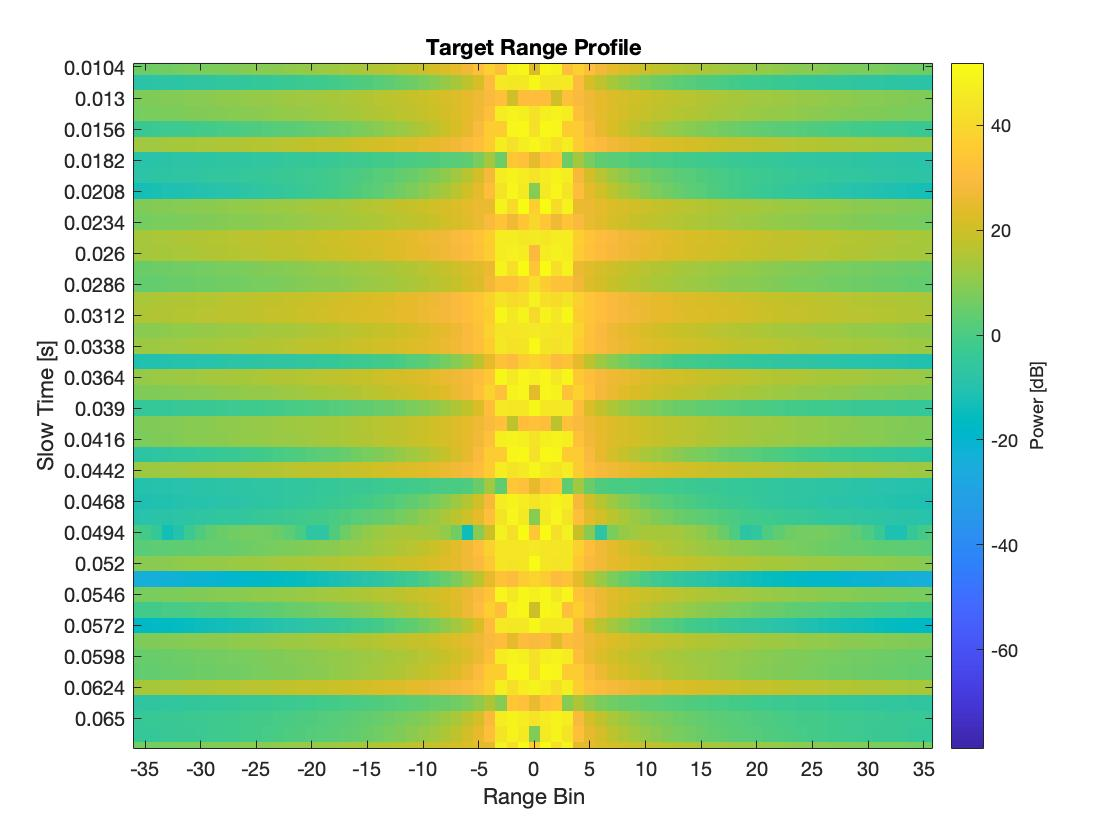
\includegraphics[width=9cm]{FMCW mD analysis-chap4/img/DJI Air 2_rt_unique.jpg}
\caption{Range profile of DJI Mavic Air 2 observed with unique waveform.}
\label{DJI-unique-wave-rt}
\end{figure}

In this lucky case, the initial phase of the different rotors allow all typical characteristics to be measured except the number of rotors. The measured distance between two blade flashes of the same rotor is 4 pixels in time, resulting in a measured period of $T_{migr} = 0.0052s$ compared to the real value of $T_{migr} = 0.0055s$. The measured range pixels on a blade flash are 4, corresponding to a migration $R_{migr}=4m$ from which we obtain a maximum blade tip speed of $v_{tip} = 51.2466 m/s$. The information of even blades is extracted and assuming that they are $N_b = 2$ and by adding it to the knowledge of $T_{BF}$ the resulting rotation rate measured is $\Omega = 604.15 rad/s$. The resulting blade length measured is $L = 0.08 m$ while the real blade length is $ L = 0.07 m$.
Making the same computation for the DJI Matrice 300 the measured distance between two blade flashes of the same rotor is 6 pixels in time, resulting in a measured period of $T_{migr} = 0.0078s$ compared to the real value of $T_{migr} = 0.0071s$. The measured range pixels on a blade flash are 9, corresponding to a migration $R_{migr}=9m$ from which we obtain a maximum blade tip speed of $v_{tip} = 115.3 m/s$. In the same way as previous the resulting rotation rate measured is $\Omega = 402.76 rad/s$. The resulting blade length measured is $L = 0.286 m$ while the real blade length is $ L = 0.2665 m$.\\
For what concern the DJI Panthom 4, the measured distance between two blade flashes of the same rotor is 6 pixels in time, resulting in a measured period of $T_{migr} = 0.0078s$ compared to the real value of $T_{migr} = 0.0071s$. The measured range pixels on a blade flash are 9, corresponding to a migration $R_{migr}=9m$ from which we obtain a maximum blade tip speed of $v_{tip} = 115.3 m/s$. In the same way as previous the resulting rotation rate measured is $\Omega = 402.76 rad/s$. The resulting blade length measured is $L = 0.286 m$ while the real blade length is $ L = 0.2665 m$.\\
In the case of DJI Panthom 4, the result obtain are always a continuous band of balde flashes as shown in figure \ref{DJI-panthom-unique-wave-rt}. This is due to the fact that its blade flash period is too small, it is only $T_{BF} = 0.0043s$ and it is the smaller one among the analyzed drones. In this case it is only possible to measure the blade tip velocity of the drone, as seen in figure the number of pixel migrated are corresponding to a migration $R_{migr}=9m$ from which we obtain a maximum blade tip speed of $v_{tip} =  38.43 m/s$. The real one is $v_{tip} =  36.44 m/s$.

\begin{figure}[h!]
\centering
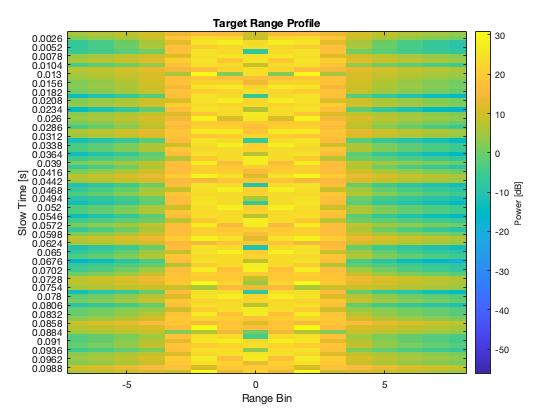
\includegraphics[width=9cm]{FMCW mD analysis-chap4/img/DJI_Panthom_4_rho_t_unique.jpg}
\caption{Range profile of DJI Panthom 4 observed with unique waveform.}
\label{DJI-panthom-unique-wave-rt}
\end{figure}


\subsubsection{Freqeuncy-time analysis}
In the table \ref{tab:ft-trex450result}, \ref{tab:ft-trex500result} and \ref{tab:ft-trex600result} are shown the result of waveform design algorithm applied with the usual radar parameters to the helicopter drones analyzed. In this case the same importance is given to the frequency and time resolution. In case of the T-Rex 500 the ambiguous range limit must be decreased from $k = 10$ times the maximum delay measured to $k = 9$ times. In \ref{tab:ft-trex600result} this limit must be decreased further to $k = 8$. This is due to the very high blade tip speeds, which require a shorter chirp duration to be measured.  In fact, the speeds reported in the drone's specifications are the maximum possible, usually in normal conditions they are lower.

\begin{table}[h!]
\centering
\begin{tabular}{|c|c|c|c|c|c|c|}
\hline
$N_{fft}$ & $T_{chirp}$ & \$f & $\Delta f$ & $P_{tx}$ & S & $f_{ADC}$ \\ \hline
20 & 101.64$\mu$s & 491 Hz & 1 ms & 31.4 W & 1474 GHz/s & 19.6 MHz \\ \hline
28 & 81.16 $\mu$s & 440 Hz & 1.1 ms & 28.1 W & 1846 GHz/s & 24.65 MHz \\ \hline
36 & 69.4 $\mu$s & 400 Hz & 1.3 ms & 25.5 W & 2158 GHz/s & 28.8 MHz \\ \hline
44 & 71 $\mu$s & 320 Hz & 1.6 ms & 20.4 W & 2110 GHz/s & 28.1 MHz \\ \hline
52 & 68.68 $\mu$s & 280 Hz & 1.8 ms & 17.8 W & 2182 GHz/s & 29.1 MHz \\ \hline
60 & 69.4 $\mu$s & 250 Hz & 2.1 ms & 15.3 W & 2158 GHz/s & 28.8 MHz \\ \hline
68 & 73.52 $\mu$s & 200 Hz & 2.5 ms & 12.7 W & 2038 GHz/s & 27.2 MHz \\ \hline
\end{tabular}
\caption{Radar parameters result for T-rex 450 drone model.}
\label{tab:ft-trex450result}
\end{table}


\begin{table}[h!]
\centering
\begin{tabular}{|c|c|c|c|c|c|c|}
\hline
$N_{fft}$ & $T_{chirp}$ & \$f & $\Delta f$ & $P_{tx}$ & S & $f_{ADC}$ \\ \hline
20 & 61.3$\mu$s & 815Hz & 0.61ms & 39.4W & 2445GHz/s & 32.64MHz \\ \hline
28 & 61.3$\mu$s & 582Hz & 0.85ms & 28.1W & 2445GHz/s & 32.64MHz \\ \hline
36 & 60.38$\mu$s & 460Hz & 1.08ms & 22.2W & 2482GHz/s & 33.13MHz \\ \hline
44 & 61.3$\mu$s & 370Hz & 1.34ms & 17.9W & 2445GHz/s & 32.6MHz \\ \hline
52 & 61.3$\mu$s & 313Hz & 1.59ms & 15.1W & 2445GHz/s & 32.6MHz \\ \hline
60 & 60.38$\mu$s & 276Hz & 1.81ms & 13.3W & 2482GHz/s & 33.1MHz \\ \hline
68 & 61.3$\mu$s & 239Hz & 2.08ms & 11.5W & 2445GHz/s & 32.64MHz \\ \hline
\end{tabular}
\caption{Radar parameters result for T-rex 500 drone model.}
\label{tab:ft-trex500result}
\end{table}

\begin{table}[h!]
\centering
\begin{tabular}{|c|c|c|c|c|c|c|}
\hline
$N_{fft}$ & $T_{chirp}$ & \$f & $\Delta f$ & $P_{tx}$ & S & $f_{ADC}$ \\ \hline
20 & 55.22 $\mu$s & 905 Hz & 0.55 ms & 57.8 W & 2714 GHz/s & 36.2 MHz \\ \hline
28 & 55.22$\mu$s & 646Hz & 0.77ms & 41.3 W & 2714GHz/s & 36.23MHz \\ \hline
36 & 53.41$\mu$s & 520Hz & 0.96ms & 33.2 W & 2806GHz/s & 37.4MHz \\ \hline
44 & 55.22$\mu$s & 414Hz & 1.2ms & 26.4W & 2734GHz/s & 36.5MHz \\ \hline
52 & 53.41$\mu$s & 316.9Hz & 1.3ms & 23W & 2806GHz/s & 37.4MHz \\ \hline
60 & 55.22$\mu$s & 305Hz & 1.63ms & 19.5W & 2749GHz/s & 36.6MHz \\ \hline
68 & 55.22$\mu$s & 270Hz & 1.84ms & 17.3W & 2761GHz/s & 36.86MHz \\ \hline
\end{tabular}
\caption{Radar parameters result for T-rex 600 drone model.}
\label{tab:ft-trex600result}
\end{table}

Applying the unique waveform designed for the f-t plane: $T_{chirp} = 66.7 \mu s$, $T_{dwell} = 0.08s$ and $N_{fft} = 12 $ to the three different helicopter drones yields the following results.
First, the radar parameters with this waveform configuration are:

\begin{itemize}

    \item $t_{renew} = 6 s$ is the scan time,
    
    \item $\Delta f = 1249 Hz$ is the achieved frequency resolution,
    
    \item $\Delta t = 0.2 ms$ is the achieved time resolution due to the $75\%$ overlapping windows,
    
    \item $d = 0.40 m$ is the required antenna dimension,
         
    \item $\theta_{az} = 4.8\degree$ is the required azimuth resolution,

    \item $P_{tx} = 14.53 W$ is the necessary transmitted power,
    
    \item $S = 2247 GHz/s$ is the required chirp slope,
    
    \item $f_{ADC} = 30 MHz$ is the required sampling frequency.
    
    \item $R_{max} = 1000 m$ is the maximum identification range for a helicopter drone.

    
\end{itemize}

As visual example the T-Rex 450 spectrogram is shown in figure \ref{t-rex-unique-wave-ft}. It possible to observe more than 5 blade flashes due to the fact that the blade flash period for this drone is $T_{BF} = 0.0125 s$. The max frequency measured from the spectrogram is $4997.5 Hz$ instead of $4904.3 Hz$, that is an acceptable result. The number of time pixels measured between 2 blade flash is $62$, resulting in a measured period of $T_{BF} = 0.0125s$ compared to the real value of $T_{BF} = 0.0125s$. By extracting the number of blades information $N_{b} = 2$ it's possible to compute the rotation rate $\Omega = 253.35 rad/s$. From the maximum frequency the blade tip velocity  is $v_{tip}=83.23 m/s$ and the resulting blade length extracted is $L=0.328m$ while the real value is $L = 0.325m$.

\begin{figure}[h!]
\centering
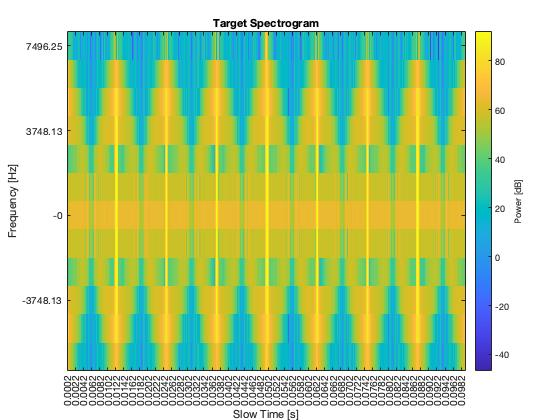
\includegraphics[width=12cm]{FMCW mD analysis-chap4/img/trex450_result_spect_unique_waveform.jpg}
\caption{Spectrogram of T-Rex 450 observed with unique waveform.}
\label{t-rex-unique-wave-ft}
\end{figure}

In the case of T-Rex 500 the maximum measured frequency from the spectrum is $7496 Hz$ instead of the real one $8.156Hz$. This is a limitation of the designed waveform, but considering that such very high speed of rotation for the helicopter drones are dangerous and usually the rotation rate are lower we can accept it. The number of time pixels measured between 2 blade flash is $54$, resulting in a measured period of $T_{BF} = 0.0108s$ compared to the real value of $T_{BF} = 0.0109s$. By extracting the number of blades information $N_{b} = 2$ it's possible to compute the rotation rate $\Omega = 290.88 rad/s$. From the maximum frequency the blade tip velocity is $v_{tip}= 124.84 m/s$ and the resulting blade length extracted is $L=0.429m$ while the real value is $L = 0.47m$.

%aggiugnere calcoli anche qui

Also for the case of T-Rex 600 the max measured frequency is affected by the same problem, it is $7496 Hz$, and it is the maximum one that the radar can measure. While the real max frequency is $9054 Hz$. The number of time pixels measured between 2 blade flash is $62$, resulting in a measured period of $T_{BF} = 0.0124s$ compared to the real value of $T_{BF} = 0.0125s$. By extracting the number of blades information $N_{b} = 2$ it's possible to compute the rotation rate $\Omega = 253.35 rad/s$. From the maximum frequency the blade tip velocity is $v_{tip}= 124.84 m/s$ and the resulting blade length extracted is $L=0.5m$ while the real value is $L = 0.6m$. 

In the table \ref{tab:dji-air2-result}, \ref{tab:dji-matrice300-result} and \ref{tab:dji-panthom4-result} are shown the result of waveform design algorithm applied with the usual radar parameters to the quadcopter drones. In this case the same importance is given to the frequency and time resolution. The scan time is set to $t_{renew} = 2s $. In case of DJI Panthom 4 the required minimum pixel in time and frequency between two blade flash must be decreased to $n_t = 4$ and $n_f = 4$ in order to respect all the chirp limitations.\\

\begin{table}[h!]
\centering
\begin{tabular}{|c|c|c|c|c|c|c|}
\hline
$N_{fft}$ & $T_{chirp}$ & $\Delta_f$ & $\Delta_t$ & $P_{tx}$ & S & $f_{ADC}$ \\ \hline
12 & 181.95$\mu$s & 458Hz & 1.09ms & 16.74W & 823.8GHz/s & 10.99MHz \\ \hline
16 & 136.46$\mu$s & 458Hz & 1.09ms & 16.74W & 1098GHz/s & 14.66MHz \\ \hline
20 & 109.17$\mu$s & 458Hz & 1.09ms & 16.74W & 1373GHz/s & 18.32MHz \\ \hline
24 & 90.97$\mu$s & 458Hz & 1.09ms & 16.74W & 1647GHz/s & 21.98MHz \\ \hline
28 & 77.97$\mu$s & 458Hz & 1.09ms & 16.74W & 1922GHz/s & 29.1 MHz \\ \hline
32 & 68.23$\mu$s & 458Hz & 1.09ms & 16.74W & 2196GHz/s & 29.31MHz \\ \hline
\end{tabular}
\caption{Radar parameters result for DJI Mavic Air 2 drone model.}
\label{tab:dji-air2-result}
\end{table}

\begin{table}[h!]
\centering
\begin{tabular}{|c|c|c|c|c|c|c|}
\hline
$N_{fft}$ & $T_{chirp}$ & $\Delta_f$ & $\Delta_t$ & $P_{tx}$ & S & \$f\_\{ADC\} \\ \hline
12 & 71.04$\mu$s & 1172Hz & 0.42ms & 73.42W & 2109GHz/s & 28.16MHz \\ \hline
16 & 71.04$\mu$s & 879Hz & 0.56ms & 55.06W & 2109GHz/s & 28.16MHz \\ \hline
20 & 71.04$\mu$s & 703Hz & 0.71ms & 44.05W & 2109GHz/s & 28.16MHz \\ \hline
24 & 71.04$\mu$s & 586Hz & 0.85ms & 36.71W & 2109GHz/s & 28.16MHz \\ \hline
28 & 71.04$\mu$s & 502Hz & 0.99ms & 31.46W & 2109GHz/s & 28.16MHz \\ \hline
32 & 71.04$\mu$s & 439Hz & 1.13ms & 27.53W & 2109GHz/s & 28.16MHz \\ \hline
\end{tabular}
\caption{Radar parameters result for DJI Matrice 300 drone model.}
\label{tab:dji-matrice300-result}
\end{table}

\begin{table}[h!]
\centering
\begin{tabular}{|c|c|c|c|c|c|c|}
\hline
$N_{fft}$ & $T_{chirp}$ & $\Delta_f$ & $\Delta_t$ & $P_{tx}$ & S & \$f\_\{ADC\} \\ \hline
12 & 179.59$\mu$s & 464Hz & 1.07ms & 10.57W & 834 GHz/s & 11.14MHz \\ \hline
16 & 134.69$\mu$s & 464Hz & 464ms & 10.57W & 1112GHz/s & 14.85MHz \\ \hline
20 & 107.75$\mu$s & 464Hz & 464ms & 10.57W & 1391GHz/s & 18.56MHz \\ \hline
24 & 89.79$\mu$s & 464Hz & 464ms & 10.57W & 1669GHz/s & 22.27MHz \\ \hline
28 & 76.97$\mu$s & 464Hz & 464ms & 10.57W & 1947GHz/s & 25.98MHz \\ \hline
32 & 67.34$\mu$s & 439Hz & 1.13ms & 10.57W & 2225GHz/s & 29.7MHz \\ \hline
\end{tabular}
\caption{Radar parameters result for DJI Panthom 4 drone model.}
\label{tab:dji-panthom4-result}
\end{table}


Applying the unique waveform designed for the f-t plane: $T_{chirp} = 66.7 \mu s$, $T_{dwell} = 0.8s$ and $N_{fft} = 12 $ to the three different quadcopter drones yields the following results.
First the radar parameters with this waveform configuration are:

\begin{itemize}

    \item $t_{renew} = 6 s$ is the scan time,
    
    \item $\Delta f = 1249 Hz$ is the achieved frequency resolution,
    
    \item $\Delta t = 0.2 ms$ is the achieved time resolution due to the $75\%$ overlapping windows,
    
    \item $d = 0.40 m$ is the required antenna dimension,
         
    \item $\theta_{az} = 4.8\degree$ is the required azimuth resolution,

    \item $P_{tx} = 17.86 W$ is the necessary transmitted power,
    
    \item $S = 2247 GHz/s$ is the required chirp slope,
    
    \item $f_{ADC} = 24 MHz$ is the required sampling frequency.
    
    \item $R_{max} = 800 m$ is the maximum identification range for a quadcopter drone.

\end{itemize}


As visual example the DJI Mavic Air 2 spectrogram is shown in figure \ref{djimavic2-unique-wave-ft}.


\begin{figure}[h!]
\centering
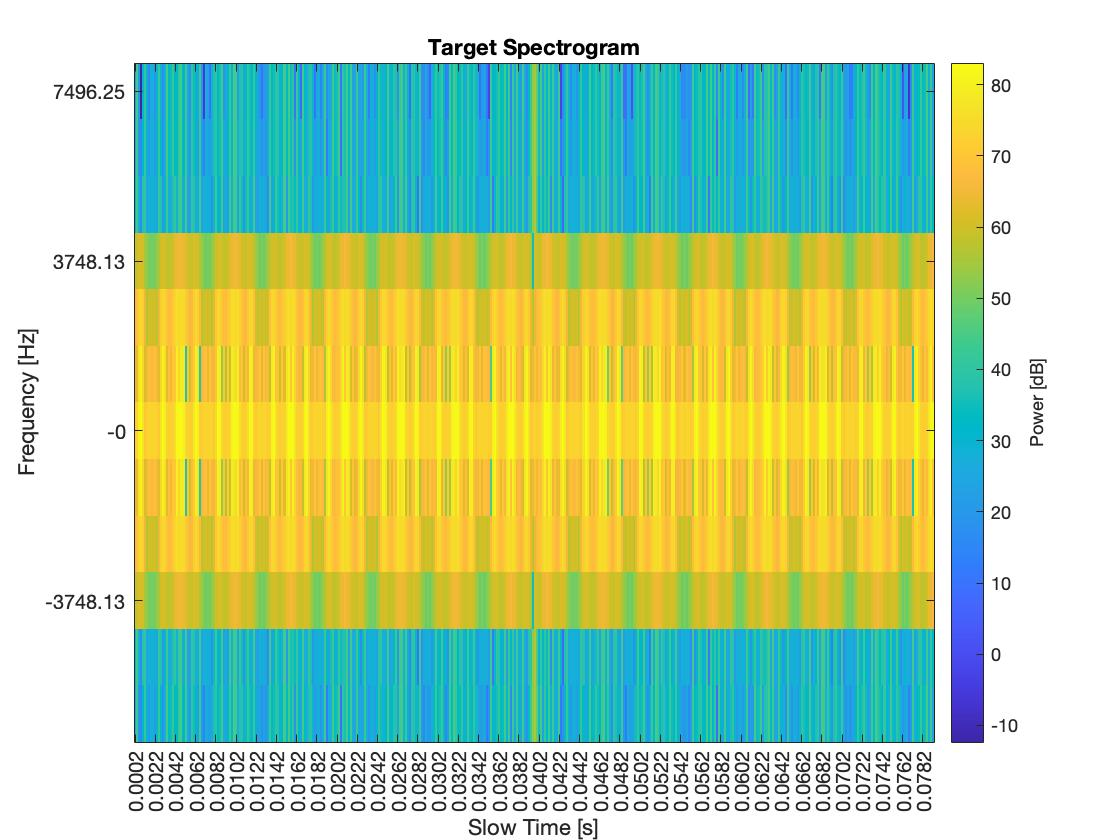
\includegraphics[width=12cm]{FMCW mD analysis-chap4/img/dji_mavic_2_quad_ft_unique.jpg}
\caption{Spectrogram of DJI Mavic Air 2 observed with unique waveform.}
\label{djimavic2-unique-wave-ft}
\end{figure}

The max frequency measured from the spectrogram is $2498 Hz$ instead of $2418 Hz$. The number of time pixels measured between 2 blade flash of the same rotor is $27$, resulting in a measured period of $T_{BF} = 0.0054s$ compared to the real value of $T_{BF} = 0.0055s$. By extracting the number of blades information $N_{b} = 2$ it's possible to compute the rotation rate $\Omega = 581.77 rad/s$. From the maximum frequency the $v_{tip}=41.60 m/s$ and the resulting blade length extracted is $L=0.0715m$ while the real value is $L = 0.07m$.\\
Making the same computation for the DJI matrice 300 model, the max frequency measured from the spectrogram is $7496 Hz$ instead of $7037 Hz$. In this case, it can be seen how the frequency resolution leads to a result with a deviation from the true value of approximately $459.66Hz$. The number of time pixels measured between 2 blade flash of the same rotor is $35$, resulting in a measured period of $T_{BF} = 0.0070s$ compared to the real value of $T_{BF} = 0.0071s$. By extracting the number of blades information $N_{b} = 2$ it's possible to compute the rotation rate $\Omega = 448.79 rad/s$. From the maximum frequency the $v_{tip}=124.84 m/s$ and the resulting blade length extracted is $L=0.278m$ while the real value is $L = 0.2665m$.\\
Making the same computation for the last quadcopter drone, the DJI Panthom 4 model, the max frequency measured from the spectrogram is $2498 Hz$ instead of $2188 Hz$. The number of time pixels measured between 2 blade flash of the same rotor is $22$, resulting in a measured period of $T_{BF} = 0.0044s$ compared to the real value of $T_{BF} = 0.0043s$. By extracting the number of blades information $N_{b} = 2$ it's possible to compute the rotation rate $\Omega = 713.99 rad/s$. From the maximum frequency the $v_{tip}=41.6 m/s$ and the resulting blade length extracted is $L=0.058m$ while the real value is $L = 0.05m$.

\subsection{Summary}
Final considerations are now made on the results obtained. Particular attention is given to the required power and then which of the two analyses, the Frequency-Time one or the Range-Time one, is more convenient will be analysed later knowing first the final energy and radar parameters balance. As seen in the previous section the information that can be extracted in both analyses are considered satisfactory. In fact, these allow to measure the length of the drone's blades with an accuracy of the order of millimetres, and the blade flash period with an accuracy in the order of tenth of millisecond. On the other hand the main problem that must be avoided, as seen in the radar parameters, is the too high power requirements. There are six possible solutions in order to decrease the power:

\begin{itemize}

    \item Decrease the carrier frequency $f_{c}$,

    \item Increase the renewal time $t_{renew}$,
    
    \item Decrease the dwell time $t_{dwell}$,
    
    \item Decrease the max Range $R_{max}$,
    
    \item Assume a lower Noise Figure $L$,
         
    \item Decrease the $SNR_{min}$ required.

\end{itemize}

By decreasing the frequency and moving into the S-band, the resulting wavelength becomes larger, which results in a much lower power requirement. On the other hand, a wavelength in the range of $0.07-0.14 cm$ does not allow the basic assumption of the scattering centre model to be correctly applied. As a result, there will be few reflective points forming the drone, not leading to converging towards a result similar to the real one.\\
Decreasing the renewal time could be an acceptable solution, but only up to a certain time limit. In fact, considering the average speeds of drones and the maximum range of around 1000m, the presence of the drone could be detected too late.\\
Decreasing the maximum range is not an option considering that it is one of the main objectives to have at least 1 km of coverage.\\
The dwell time is a parameter that can certainly be decreased, sometimes it is also necessary not to have a dwell time above a certain level, as in the case of multifunctional radars. In this regard, for the purposes of feature extraction and classification, it is also possible to observe only two blade flashes. This decreases the minimum required observation time by more than a factor of two, making the power required far less.\\
It is certainly possible to work on the quality of the constituent components of the radar and assume a total resulting noise figure of around $7 dB$ rather than $10 dB$, as done in the work \cite{MartinMulgrew}.\\
The minimum $SNR$ required to perform the coarse identification can also be relaxed, with the Swerling 0 condition being used rather than the Swerling 1-2 condition, resulting in a minimum $SNR$ of $13.2 dB$ rather than $20 dB$.\\
The final choice to decrease the required power therefore falls on the observation time and the Swerling 0 condition for the minimum $SNR$. A noise figure of $7 dB$ is assumed. In this case we have the following final parameters for the radar considering the unique waveform designed for the two analyses. In the Range-Time analysis by adding these last considerations the final energy-radar parameters balance is:

\begin{itemize}

    \item $T_{chirp} = 1.3ms$ is the chirp duration,
    
    \item $t_{dwell} = 0.04s$ is the observation time,
    
    \item $t_{renew} = 2 s$ is the scan time,

    \item $d = 0.3 m$ is the required antenna dimension,
         
    \item $\theta_{az} = 7.2\degree$ is the required azimuth resolution,

    \item $P_{tx} = 6.32 W$ is the necessary transmitted power,
    
    \item $S = 115.3 GHz/s$ is the required chirp slope,
    
    \item $f_{ADC} = 1.55 MHz$ is the required sampling frequency.
    
    \item $R_{max} = 1000 m$ is the maximum identification range.

    
\end{itemize}

In this case, all the most stringent parameters between the two drone models, quadcopter and helicopter, were considered. For example, the required power shown is that of the quadcopter drone, which has a lower RCS. In fact, for a helicopter drone is necessary $P_{tx} = 2.1 W$.\\
In the Frequency-Time analysis the final energy-radar parameters balance is:

\begin{itemize}
    
    \item $T_{chirp} = 66.7 \mu s$ is the chirp duration,
    
    \item $\Delta f = 1249 Hz$ is the achieved frequency resolution,
    
    \item $\Delta t = 0.4 ms$ is the achieved time resolution,
    
    \item $t_{dwell} = 0.04s$ is the observation time,

    \item $d = 0.3 m$ is the required antenna dimension,
         
    \item $\theta_{az} = 7.2\degree$ is the required azimuth resolution,

    \item $P_{tx} = 10.27 W$ is the necessary transmitted power,
    
    \item $S = 2247 GHz/s$ is the required chirp slope,
    
    \item $f_{ADC} = 30 MHz$ is the required sampling frequency,
    
    \item $R_{max} = 1000 m$ is the maximum identification range.

    
\end{itemize}

Also in this case the parameter considered are the more stringent. The required power showed is for the quadcopter drone, while the required power for the helicopter is $P_{tx} = 3.42 W$.\\
As can be seen, the power requirements are not very different, the Range-Time analysis needs about 4 Watts less than the Frequency-Time analysis. The substantial difference is in the sampling frequency requirement, which is about 20 times lower in the Range-Time analysis. Based on these results and considering the classification results shown in the previous section, it is preferable to perform the Range-Time analysis for the application scenario characteristic of this thesis. In fact, in addition to having a sampling rate 20 times lower than the f-t analysis, the slope of the waveform is also 20 times lower. Moreover, the main task to be fulfilled by the designed radar is to distinguish a drone from any other object or bird, not to precisely identify the model. Considering that the main difference in the results obtained through the two analyses, is the temporal resolution which can create difficulties in the identification of the specific drone model and not in the generic classification. In fact, with the Range-Time analysis, it is possible to identify the observed drone model only when the initial phase of the different rotors allow it, otherwise it is only possible to measure the maximum rotational speed of the blade tip. This problem does not arise in the case of helicopter drones that have only one rotor. An additional benefit that comes at a lower cost in the case of the range profile is the processing time required. Building only the range profile of the observed target is less complex and faster than building the spectrogram. The only processing step required is the FFT of all received echoes, which can be done in parallel in an extremely short time. The last consideration concerns the results obtained in the previous section, where with the Range-Time analysis it is clearly visible how a drone can always be classified in a coarse way into two macro categories: helicopter and quadcopter. This always makes it possible to distinguish it from other objects or birds. As en example in figure \ref{md_of_owl} is shown how a spectrogram of a bird is always different from the one of drones. To make these measurements was used a pulsed radar in S-band at $2.4 GHz$. In the three spectrograms the only difference is in the antenna configuration that is monostatic HH, bistatic HH, and monostatic HV. In that images the Doppler peaks are displayed when the bird flaps its wings frequently, whereas when it moves its wings slowly or glides, only the contribution of the body is displayed. Considering that wings are moved in a completely random manner by a bird, whereas a drone has rotating blades that perform an always periodic movement, it is always possible to distinguish the two subjects by means of the micro Doppler analysis.
 
\begin{figure}[h!]
\centering
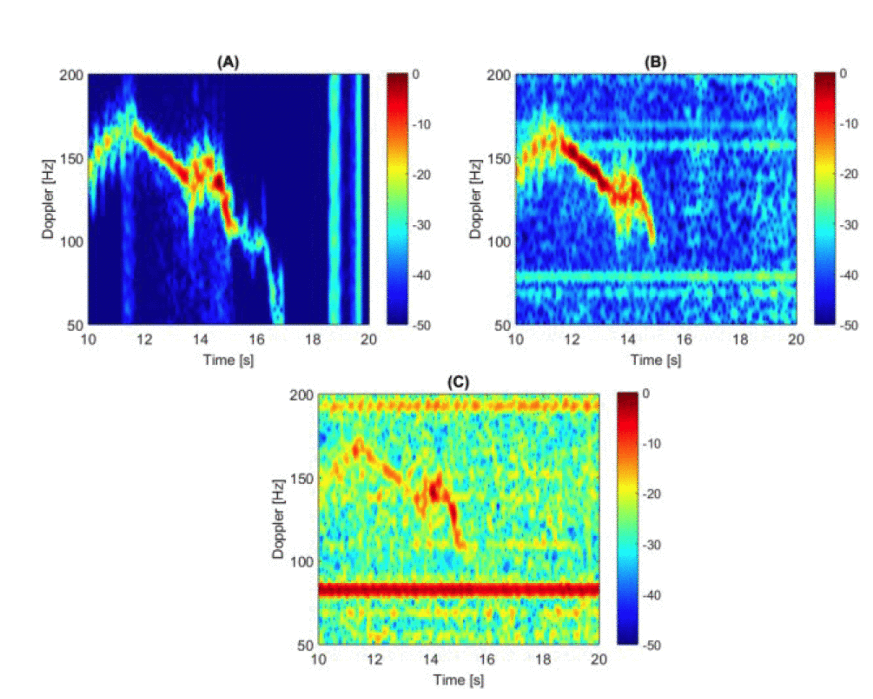
\includegraphics[width=13cm]{FMCW mD analysis-chap4/img/md of owl.png}
\caption{Micro Doppler of owl observed with different antenna configurations. \cite{md_of_owl}}
\label{md_of_owl}
\end{figure}
Therefore, by selecting to carry out the analysis on the Range-Time plane, all the benefits listed so far are obtained and it is possible to satisfy the main distinction task at a lower cost than the analysis conducted on the frequency time plane.
